\documentclass[12pt,a4paper,twoside]{report}
\usepackage[margin=1in]{geometry}
\setlength{\headheight}{15pt}

\usepackage[english]{babel}
\usepackage{blindtext}

% \usepackage{xcolor}

\usepackage{fancyhdr}\pagestyle{fancy}
\fancyhf{}
\fancyhead[RE]{\it{\nouppercase{\leftmark}}}
\fancyhead[LO]{\it{\nouppercase{\rightmark}}}
\fancyhead[LE,RO]{\thepage}
\fancyfoot{}
\usepackage{emptypage}
\usepackage{setspace} %for line spacing
\setlength{\parindent}{0em}
\renewcommand{\chaptername}{}   %suppress the chapter
\usepackage[hidelinks]{hyperref}

\usepackage[utf8]{inputenc}
\usepackage{amsmath,amssymb,amsfonts}

\usepackage{graphicx}\graphicspath{{figures/}}
\usepackage{subcaption}
% \usepackage{svg}
\usepackage{float}
\usepackage{enumitem}

% \usepackage{pgfplots}
% \pgfplotsset{compat=1.15}
% \usetikzlibrary{arrows}
% \usepackage{tikz}

% \definecolor{zzttqq}{rgb}{0.6,0.2,0}
% \definecolor{zzwwff}{rgb}{0.6,0.4,1}
% \definecolor{ttttff}{rgb}{0.2,0.2,1}
% \definecolor{wwccqq}{rgb}{0.4,0.8,0}
% \definecolor{purpleish}{rgb}{0.76,0.74,0.87}
% \definecolor{yellowish}{rgb}{1,1,0.75}
% \definecolor{redish}{rgb}{1,0.8,0.87}
% \definecolor{greenish}{rgb}{0.8,0.9,0.8}

\usepackage[square,numbers]{natbib}
\bibliographystyle{abbrv}
\usepackage[nottoc]{tocbibind}
\renewcommand\bibname{References}

% \usepackage{multirow}
% \usepackage{csquotes}

\setcounter{secnumdepth}{0}
\setcounter{tocdepth}{3}

\usepackage{authblk}
% \renewcommand*{\Authsep}{, \\ \bigskip}
% \renewcommand*{\Authand}{\\ \bigskip}
% \renewcommand*{\Authands}{\\ \bigskip}

\title{
    \Large{An attempt to Solution to} \\
    \Huge \textbf{Basic Graph Theory}\\ \bigskip
    \large{- Md. Saidur Rahman}
}

\author[ ]{
    \normalsize{Compilation by: \\ Asif Ajrof (1705092)}
}
\author[ ]{
    \normalsize{Mehedi Hasan (1705085)}
}
% \author[ ]{
%     \normalsize{yet another name (1705xxx)}
% }\author[ ]{
%     \normalsize{yet another another name (1705xxx)}
% }
\affil[ ]{
    \large{Department of Computer Science and Engineering \\
    Bangladesh University of Engineering and Technology.}
}
\date{
    \Large{June, 2022}
}

\raggedbottom   %clearing extra newlines at the end of sections/chapters

\begin{document}

\pagestyle{empty}   %no header footer	

\maketitle	
% \cleardoublepage    %for two-side. skip the even page. 

\onehalfspacing
\pagestyle{fancy}
\pagenumbering{roman}
% \cleardoublepage
\tableofcontents
% \listoffigures

\renewcommand{\abstractname}{Disclaimer}
\begin{abstract}
    The solutions in this compilation are either collected from senior's notes, a hint from a stack post, and/or our understanding. These are offered “as-is”, without warranty, and disclaiming liability for faults. If you find a correction or better solution to a problem, please contribute to make this compilation better.
\end{abstract}

\renewcommand{\abstractname}{Acknowledgement}
\begin{abstract}
    .
\end{abstract}
    
\onehalfspacing
\setlength{\parskip}{1em}
\pagenumbering{arabic}	

%================ch1======================================
\chapter{Graphs and Their Applications}\label{ch1}
\section{Exercises}
    \begin{enumerate}[leftmargin=1.5em]
      \item {
        Study your campus map and model the road network inside your campus by a graph.
        
        \begin{description}[leftmargin=0em]
           \item[Answer:] {
                {[}Do it yourself{]}
            }
        \end{description}
      }
      \item {
        Construct a graph to represent the adjacency relationship of rooms in a floor of your university building.
        
        \begin{description}[leftmargin=0em]
           \item[Answer:] {
                {[}Do it yourself{]}\\
                Some examples taken from a floor plan paper \cite{floor_plan} in Figure \ref{fig:1_2_floorplan_to_graph}
                \begin{figure}[ht]
                    \centering
                    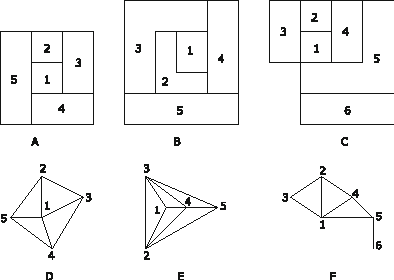
\includegraphics[width = 0.8\textwidth]{1_2_floorplan_to_graph.pdf}
                    \caption{Floor plan}
                    \label{fig:1_2_floorplan_to_graph}
                \end{figure}.
            }
        \end{description}
      }
      \item {
        Consider a party where there are exactly two alternate options of foods for each category of foods as follows. Rice: plane/yellow, Curry: fish/chicken, Naan: plain/butter, Kebab: chicken/mutton, Fruit: banana/mango, Drink: tea/coffee. Registered participants of the party gave their options as in Figure \ref{fig:1_3_table_food_opt}. Two participants conflict in their options if they give different options in the same category. Represent the conflicts of the participants using a conflict graph where each participant is represented by a vertex and there is an edge between two vertices if the corresponding participants conflict. By observing the conflict graph, find out the minimum number of persons whose absence divides the participants into two conflict free groups.
        \begin{figure}[H]
            \centering
            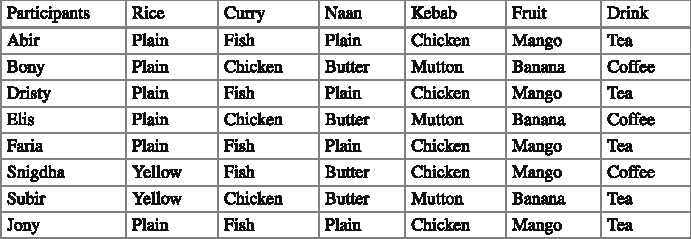
\includegraphics[width = 1\textwidth]{1_3_table_food_opt.pdf}
            \caption{Food option}
            \label{fig:1_3_table_food_opt}
        \end{figure}
        
        \begin{description}[leftmargin=0em]
           \item[Answer:] {
                Conflict graph Figure \ref{fig:1_3_conflict_graph}
                \begin{figure}[H]
                    \centering
                    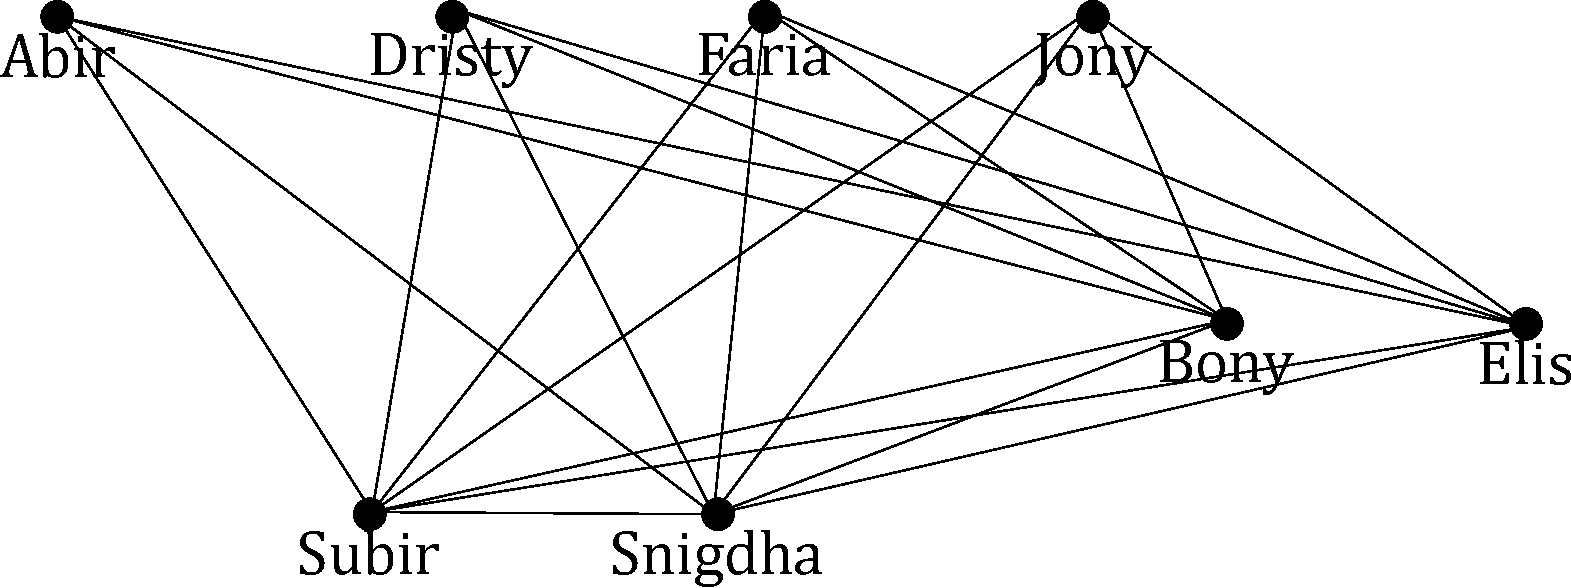
\includegraphics[width = 0.8\textwidth]{1_3_conflict_graph.pdf}
                    \caption{Conflict graph}
                    \label{fig:1_3_conflict_graph}
                \end{figure}
                
                Conflict free groups: \{Abir, Dristy, Faria, Jony\}, \{Bony, Elis\}, \{Subir\}, \{Snigdha\}.\\
                Exclude 2 persons namely Subir and Snigdha to get two conflict free groups \{Abir, Dristy, Faria, Jony\} and \{Bony, Elis\}
            }
        \end{description}
      }
      \item {
        There are five jobs $\{J_1, J_2, J_3, J_4, J_5\}$ in a company for which there are five workers $A, B, C, D$ and $E$ to do those jobs. However, everybody does not have expertise to do every job. Their expertise is as follows: $A = \{J_1, J_2, J_3\}$, $B = \{J_2, J_4\}$, $C = \{J_1, J_3, J_5\}$, $D = \{J_3, J_5\}$, $E = \{J_1, J_5\}$. Develop a graph model to represent the job expertise of the persons and find an assignment of jobs to the workers such that every worker can do a job.
        
        \begin{description}[leftmargin=0em]
           \item[Answer:] {
                Job assignment graph Figure \ref{fig:1_4_job_assg}
                \begin{figure}[H]
                    \centering
                    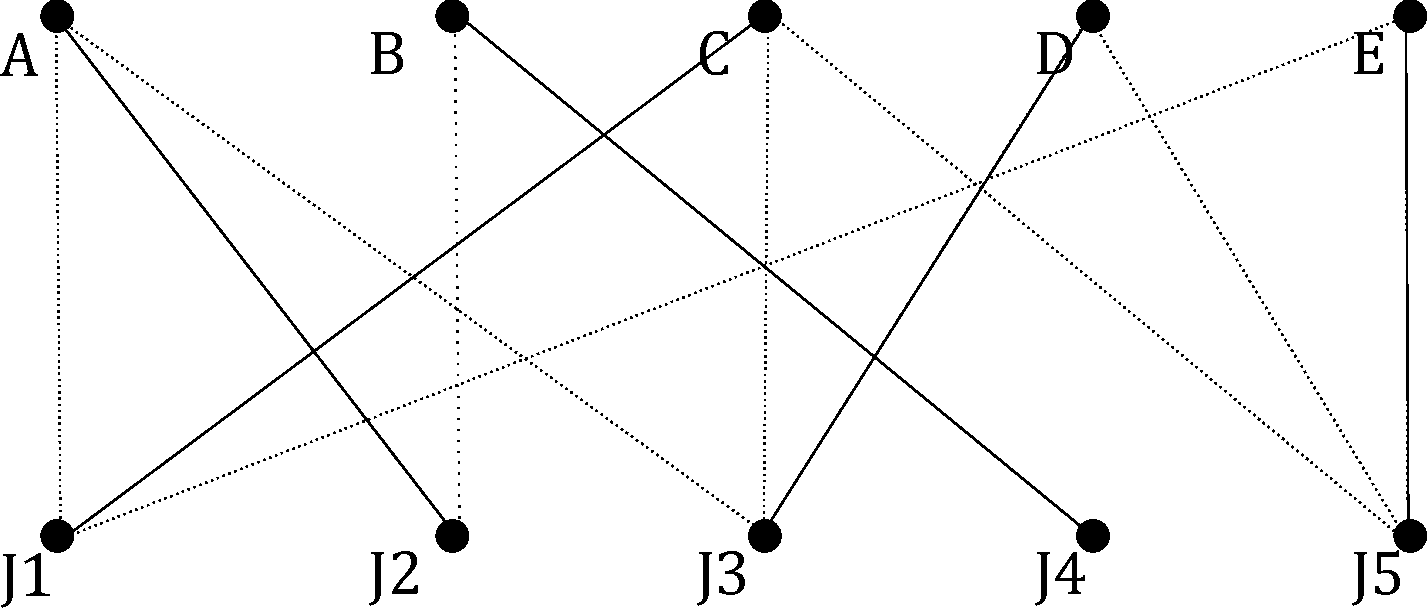
\includegraphics[width = 0.8\textwidth]{1_4_job_assg.pdf}
                    \caption{Job assignment graph}
                    \label{fig:1_4_job_assg}
                \end{figure}
            }
        \end{description}
      }
      \item {
        An industry has 600 square meter rectangular area on a floor of a building where it needs to establish four processing units $A, B, C$, and $D$. Processing units $A$ and $D$ require 100 square meter area each whereas $B$ and $C$ require 200 square meter each. Furthermore, the following adjacency requirements must be satisfied: $B, C$, and $D$ should be adjacent to $A; A$ and $D$ should be adjacent to $B; A$ and $D$ should be adjacent to $C;$ and $A, B$, and $C$ should be adjacent to $D$. Can you construct a floor layout where the space for each processing unit will be a rectangle? Propose a suitable layout in your justification.
        
        \begin{description}[leftmargin=0em]
           \item[Answer:] {
                Industry unit layout Figure \ref{fig:1_5_floor_plan}
                \begin{figure}[H]
                    \centering
                    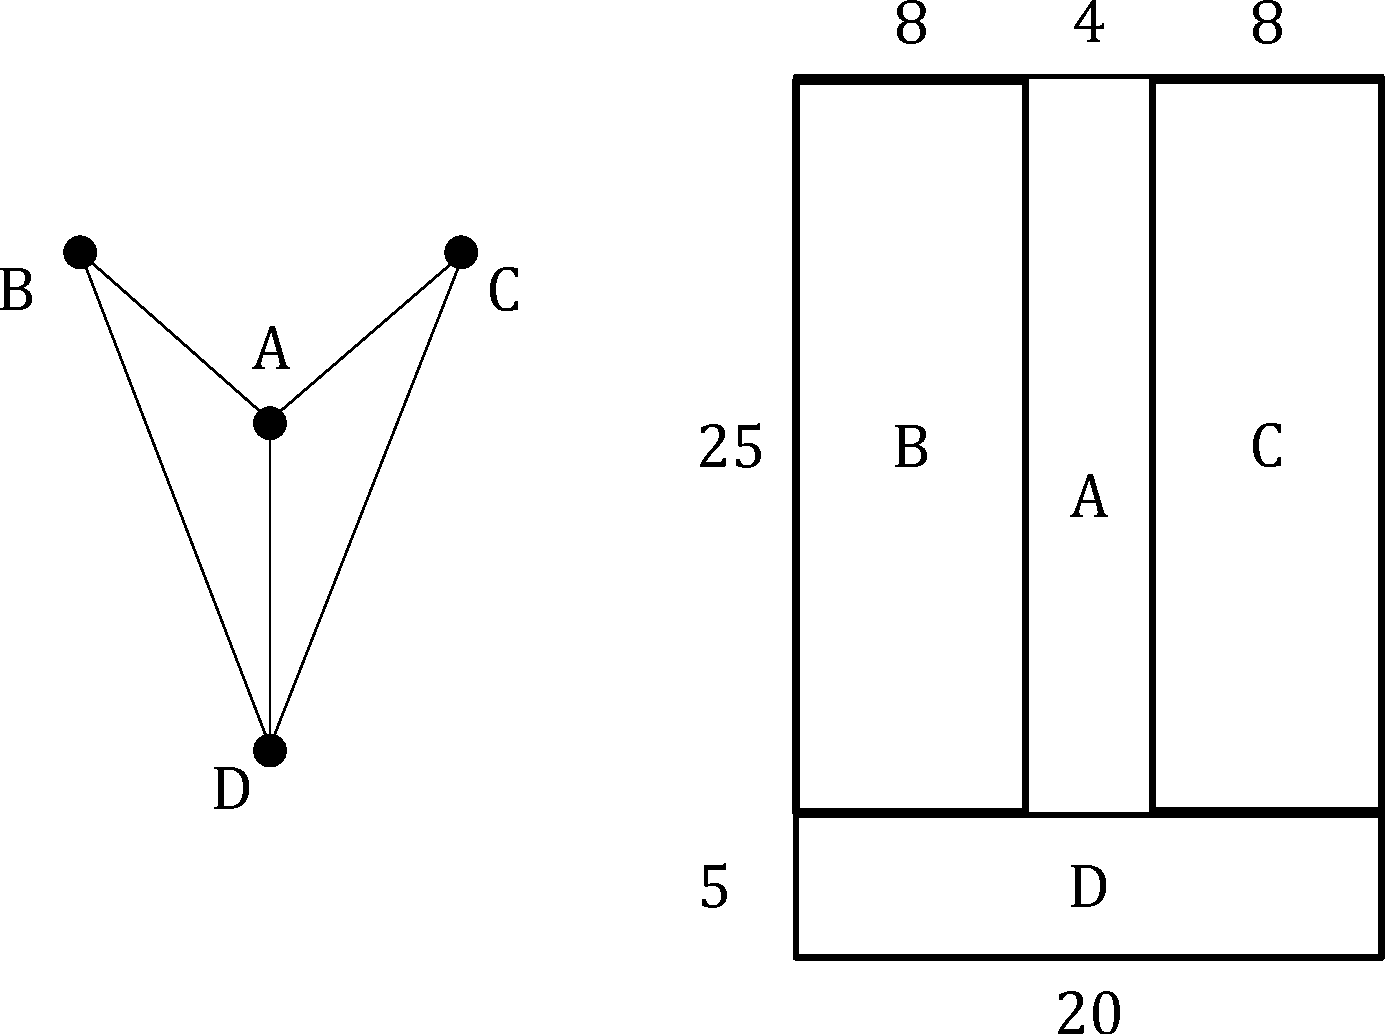
\includegraphics[width = 0.8\textwidth]{1_5_floor_plan.pdf}
                    \caption{Industry unit layout}
                    \label{fig:1_5_floor_plan}
                \end{figure}
            }
        \end{description}
      }
    \end{enumerate}
    
% \section{Solutions}
%     \begin{enumerate}[leftmargin=1.5em]
%       \item {
%         % Study your campus map and model the road network inside your campus by a graph.
        
%         \begin{description}[leftmargin=0em]
%           \item[Answer:] {
%                 {[}Do it yourself{]}
%             }
%         \end{description}
%       }
%       \item {
%         % Construct a graph to represent the adjacency relationship of rooms in a floor of your university building.
        
%         \begin{description}[leftmargin=0em]
%           \item[Answer:] {
%                 {[}Do it yourself{]}\\
%                 Some examples taken from a floor plan paper \cite{floor_plan} in Figure \ref{fig:1_2_floorplan_to_graph}
%                 \begin{figure}[ht]
%                     \centering
%                     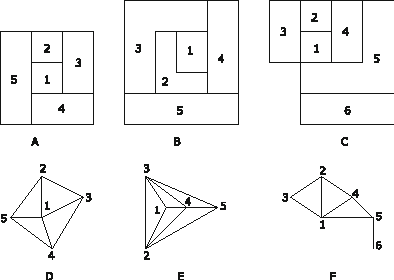
\includegraphics[width = 0.8\textwidth]{1_2_floorplan_to_graph.pdf}
%                     \caption{Floor plan}
%                     \label{fig:1_2_floorplan_to_graph}
%                 \end{figure}.
%             }
%         \end{description}
%       }
%       \item {
%         % Consider a party where there are exactly two alternate options of foods for each category of foods as follows. Rice: plane/yellow, Curry: fish/chicken, Naan: plain/butter, Kebab: chicken/mutton, Fruit: banana/mango, Drink: tea/coffee. Registered participants of the party gave their options as in Figure \ref{fig:1_3_table_food_opt}. Two participants conflict in their options if they give different options in the same category. Represent the conflicts of the participants using a conflict graph where each participant is represented by a vertex and there is an edge between two vertices if the corresponding participants conflict. By observing the conflict graph, find out the minimum number of persons whose absence divides the participants into two conflict free groups.
%         % \begin{figure}[H]
%         %     \centering
%         %     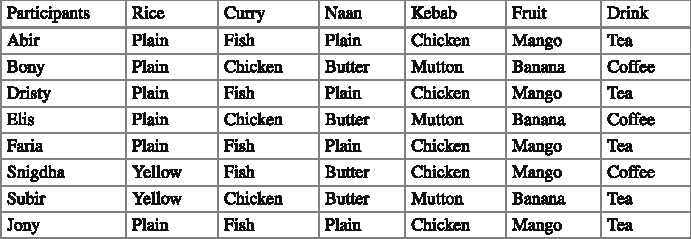
\includegraphics[width = 1\textwidth]{1_3_table_food_opt.pdf}
%         %     \caption{Food option}
%         %     \label{fig:1_3_table_food_opt}
%         % \end{figure}
        
%         \begin{description}[leftmargin=0em]
%           \item[Answer:] {
%                 Conflict graph Figure \ref{fig:1_3_conflict_graph}
%                 \begin{figure}[H]
%                     \centering
%                     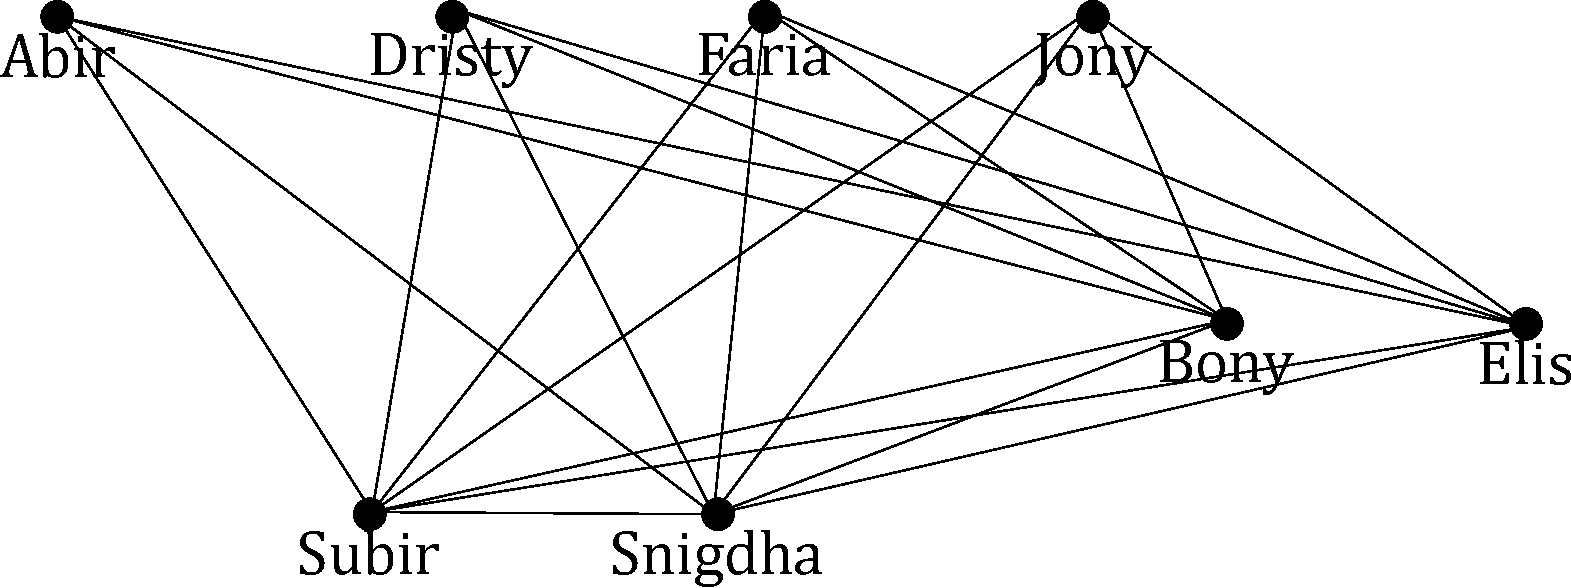
\includegraphics[width = 0.8\textwidth]{1_3_conflict_graph.pdf}
%                     \caption{Conflict graph}
%                     \label{fig:1_3_conflict_graph}
%                 \end{figure}
                
%                 Conflict free groups: \{Abir, Dristy, Faria, Jony\}, \{Bony, Elis\}, \{Subir\}, \{Snigdha\}.\\
%                 Exclude 2 persons namely Subir and Snigdha to get two conflict free groups \{Abir, Dristy, Faria, Jony\} and \{Bony, Elis\}
%             }
%         \end{description}
%       }
%       \item {
%         % There are five jobs $\{J_1, J_2, J_3, J_4, J_5\}$ in a company for which there are five workers $A, B, C, D$ and $E$ to do those jobs. However, everybody does not have expertise to do every job. Their expertise is as follows: $A = \{J_1, J_2, J_3\}$, $B = \{J_2, J_4\}$, $C = \{J_1, J_3, J_5\}$, $D = \{J_3, J_5\}$, $E = \{J_1, J_5\}$. Develop a graph model to represent the job expertise of the persons and find an assignment of jobs to the workers such that every worker can do a job.
        
%         \begin{description}[leftmargin=0em]
%           \item[Answer:] {
%                 Job assignment graph Figure \ref{fig:1_4_job_assg}
%                 \begin{figure}[H]
%                     \centering
%                     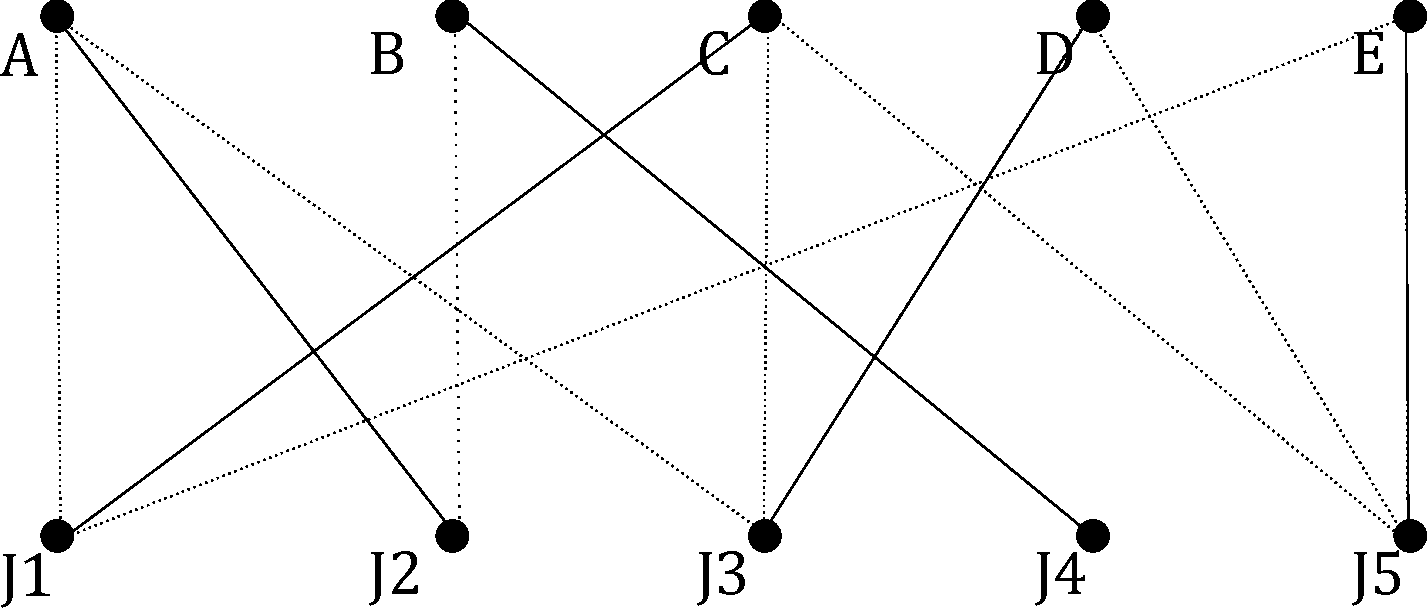
\includegraphics[width = 0.8\textwidth]{1_4_job_assg.pdf}
%                     \caption{Job assignment graph}
%                     \label{fig:1_4_job_assg}
%                 \end{figure}
%             }
%         \end{description}
%       }
%       \item {
%         % An industry has 600 square meter rectangular area on a floor of a building where it needs to establish four processing units $A, B, C$, and $D$. Processing units $A$ and $D$ require 100 square meter area each whereas $B$ and $C$ require 200 square meter each. Furthermore, the following adjacency requirements must be satisfied: $B, C$, and $D$ should be adjacent to $A; A$ and $D$ should be adjacent to $B; A$ and $D$ should be adjacent to $C;$ and $A, B$, and $C$ should be adjacent to $D$. Can you construct a floor layout where the space for each processing unit will be a rectangle? Propose a suitable layout in your justification.
        
%         \begin{description}[leftmargin=0em]
%           \item[Answer:] {
%                 Industry unit layout Figure \ref{fig:1_5_floor_plan}
%                 \begin{figure}[H]
%                     \centering
%                     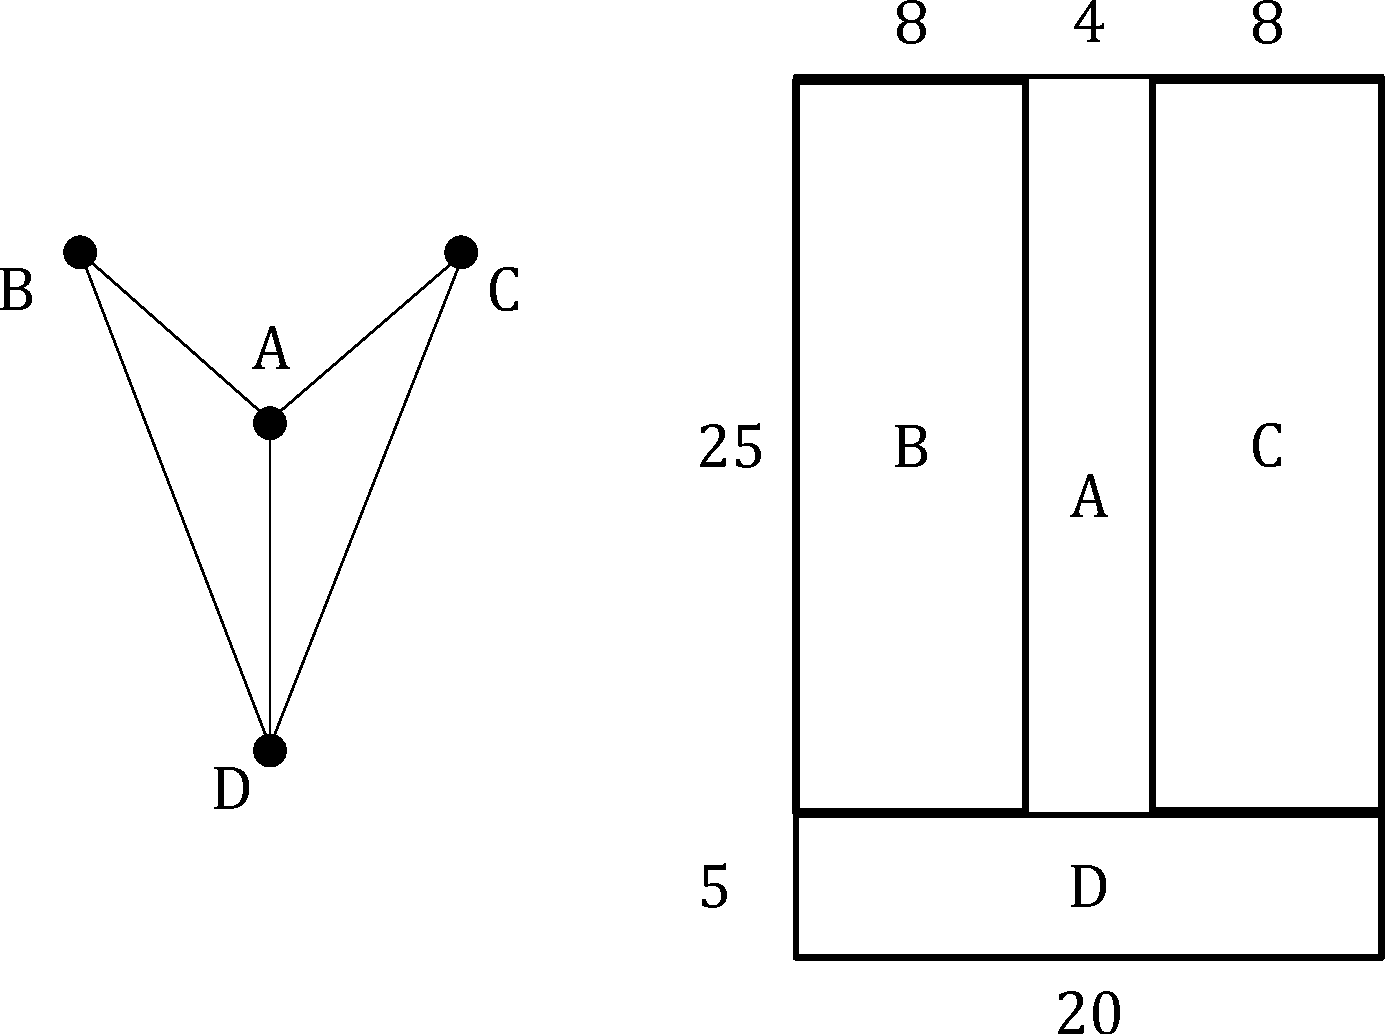
\includegraphics[width = 0.8\textwidth]{1_5_floor_plan.pdf}
%                     \caption{Industry unit layout}
%                     \label{fig:1_5_floor_plan}
%                 \end{figure}
%             }
%         \end{description}
%       }
%     \end{enumerate}

%================ch2======================================
\chapter{Basic Graph Terminologies}\label{ch2}
\section{Exercises}
    \begin{enumerate}[leftmargin=1.5em]
      \item {
        Show that every regular graph with an odd degree has an even number of vertices.
        
        \begin{description}[leftmargin=0em]
           \item[Answer:] {
                $k$-regular graph of vertices $n$, where $k$ is odd.\\
                Degree sum $= 2m$, where $m$ is number of edges.\\
                $2m = k \times n$\\
                $k$ is odd, $2m$ is even.\\
                $\therefore n$ must be even.
            }
        \end{description}
      }
      \item {
        Construct the complement of $K_{3,3}, W_{5}$, and $C_{5}$.
        
        \begin{description}[leftmargin=0em]
           \item[Answer:] {
                Complement of $K_{3,3}$ Figure \ref{fig:2_2_k}
                \begin{figure}[H]
                    \centering
                    \begin{subfigure}[b]{0.3\textwidth}
                        \centering
                        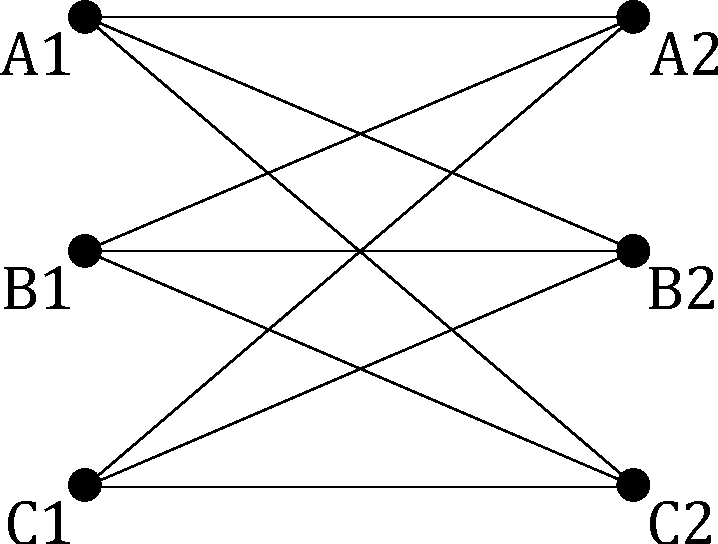
\includegraphics[width = 0.8\textwidth]{2_2_k33.pdf}
                        \caption{$K_{3,3}$}
                        \label{fig:2_2_k33}
                    \end{subfigure}
                    % \hfill
                    \begin{subfigure}[b]{0.4\textwidth}
                        \centering
                        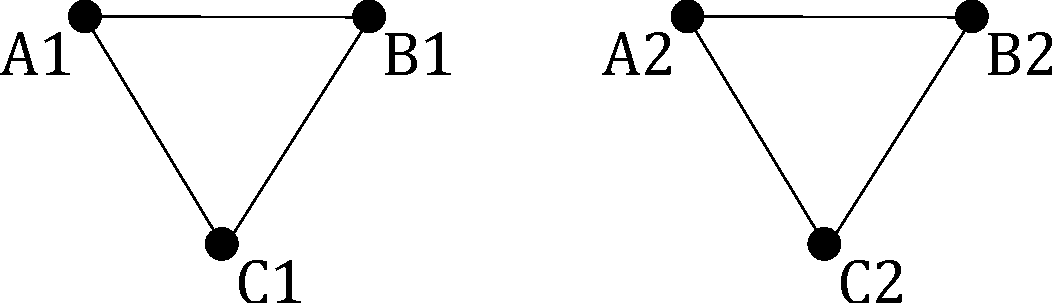
\includegraphics[width = 0.8\textwidth]{2_2_k33_c.pdf}
                        \caption{$\overline{K}_{3,3}$}
                        \label{fig:2_2_k33_c}
                    \end{subfigure}
                    \caption{Complement of $K_{3,3}$}
                    \label{fig:2_2_k}
                \end{figure}
                
                Complement of $W_{5}$ Figure \ref{fig:2_2_w}
                \begin{figure}[H]
                    \centering
                    \begin{subfigure}[b]{0.3\textwidth}
                        \centering
                        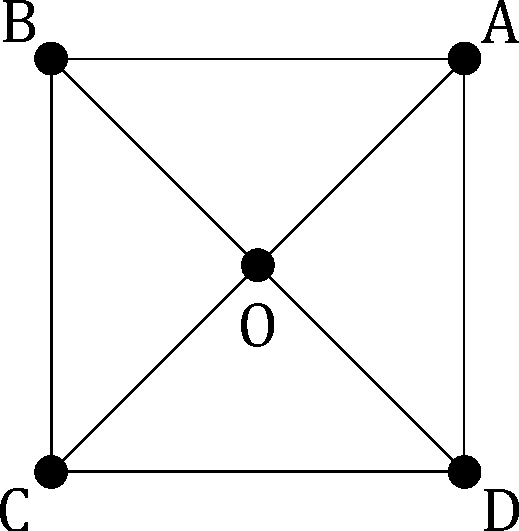
\includegraphics[width = 0.8\textwidth]{2_2_w5.pdf}
                        \caption{$W_{5}$}
                        \label{fig:2_2_w5}
                    \end{subfigure}
                    % \hfill
                    \begin{subfigure}[b]{0.4\textwidth}
                        \centering
                        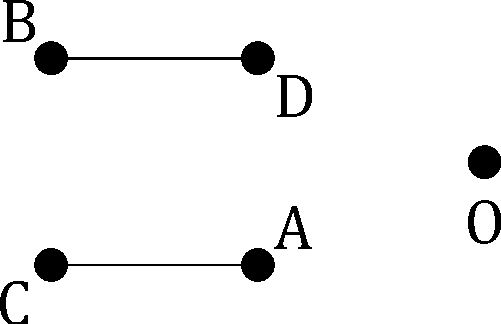
\includegraphics[width = 0.8\textwidth]{2_2_w5_c.pdf}
                        \caption{$\overline{W}_{5}$}
                        \label{fig:2_2_w5_c}
                    \end{subfigure}
                    \caption{Complement of $W_{5}$}
                    \label{fig:2_2_w}
                \end{figure}
                
                Complement of $C_{5}$ Figure \ref{fig:2_2_c}
                \begin{figure}[H]
                    \centering
                    \begin{subfigure}[b]{0.3\textwidth}
                        \centering
                        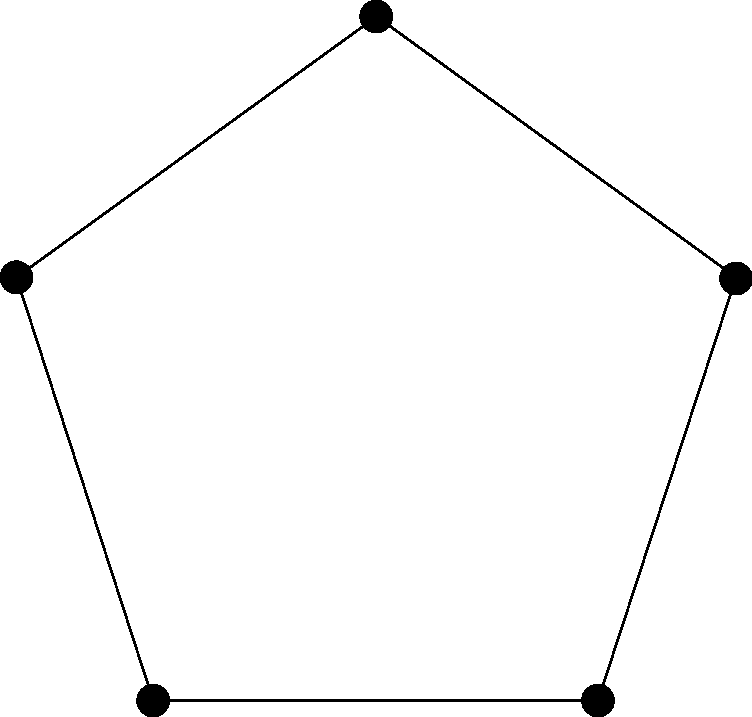
\includegraphics[width = 0.8\textwidth]{2_2_c5.pdf}
                        \caption{$C_{5}$}
                        \label{fig:2_2_c5}
                    \end{subfigure}
                    % \hfill
                    \begin{subfigure}[b]{0.3\textwidth}
                        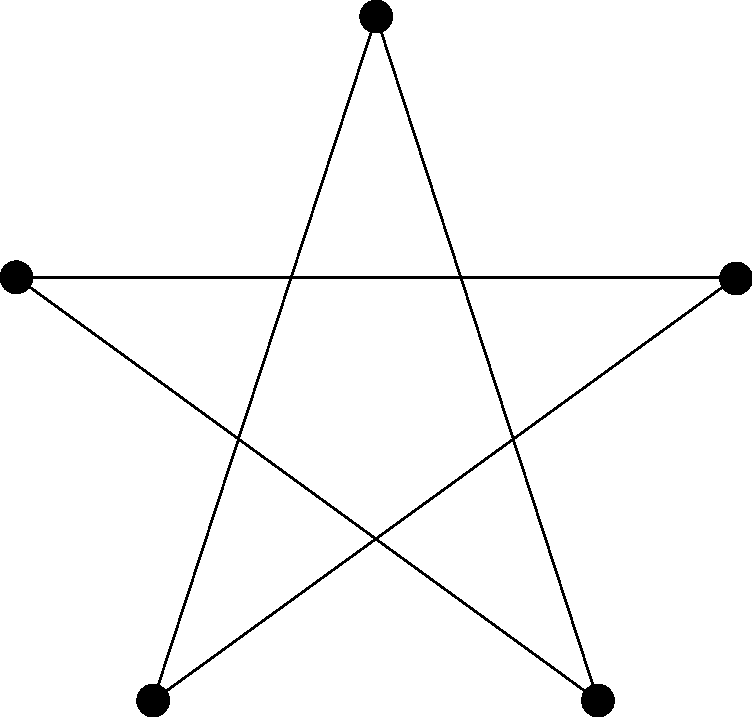
\includegraphics[width = 0.8\textwidth]{2_2_c5_c.pdf}
                        \caption{$\overline{C}_{5}$}
                        \label{fig:2_2_c5_c}
                    \end{subfigure}
                    \caption{Complement of $C_{5}$}
                    \label{fig:2_2_c}
                \end{figure}
            }
        \end{description}
      }
      \item {
        Can you construct a disconnected graph $G$ of two or more vertices such that $	\overline{G}$ is also disconnected. Give a proof supporting your answer.
        
        \begin{description}[leftmargin=0em]
           \item[Answer:] {
                No.\\
                Let us prove given a graph $G$ of two or more vertices, either $G$ or $\overline{G}$ is connected. \\
                $G$ is disconnected. We want to show that $\overline{G}$ is connected. \\
                Suppose $v$ and $w$ are vertices. If $(v, w)$ is not an edge in $G$, then it is an edge in $\overline{G}$, and so we have a path from $v$ to $w$ in $\overline{G}$. On the other hand, if $(v, w)$ is an edge in $G$, then this means $v$ and $w$ are in the same component of $G$. Since $G$ is disconnected, we can find a vertex $u$ in a different component, so that neither $(v, u)$ nor $(u, w)$ are edges of $G$. Then $(v, u, w)$ is a path from $v$ to $w$ in $\overline{G}$. \\
                This shows that any two vertices in $\overline{G}$ have a path (in fact a path of length one or two) between them in $\overline{G}$, so $\overline{G}$ is connected. \cite{122188}
                
                Example Figure \ref{fig:2_3_disc_g}:
                \begin{figure}[H]
                    \centering
                    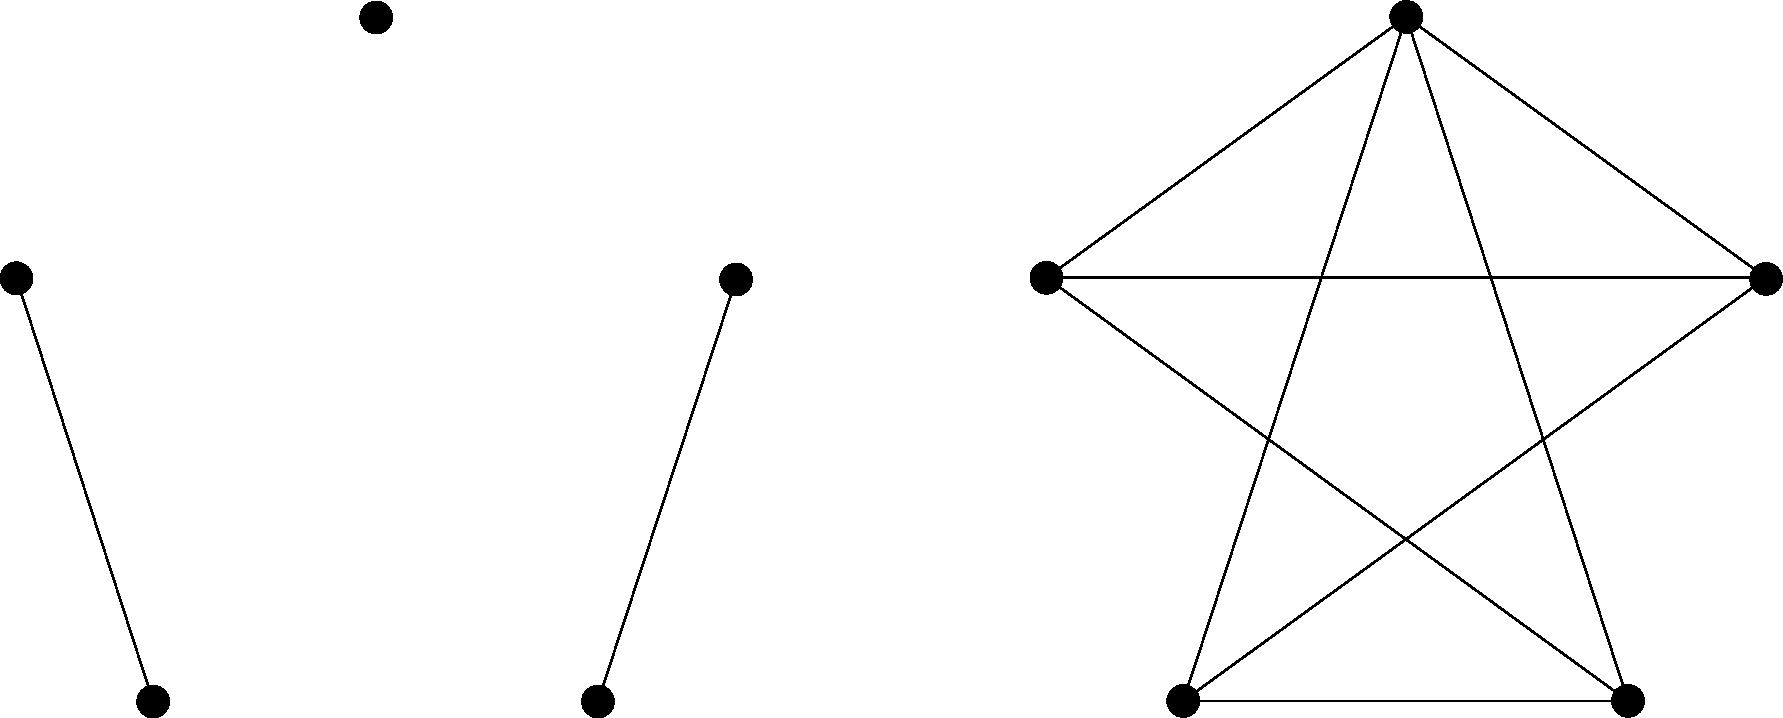
\includegraphics[width = 0.8\textwidth]{2_3_disc_g.pdf}
                    \caption{Complement of disconnected graph is connected example}
                    \label{fig:2_3_disc_g}
                \end{figure}
            }
        \end{description}
      }
      \item {
        Give two examples of self-complementary graphs.
        
        \begin{description}[leftmargin=0em]
           \item[Answer:] {
                Self complementary graphs example: $C_5$, $P_4$ Figure \ref{fig:2_4_self_compl}
                \begin{figure}[H]
                    \centering
                    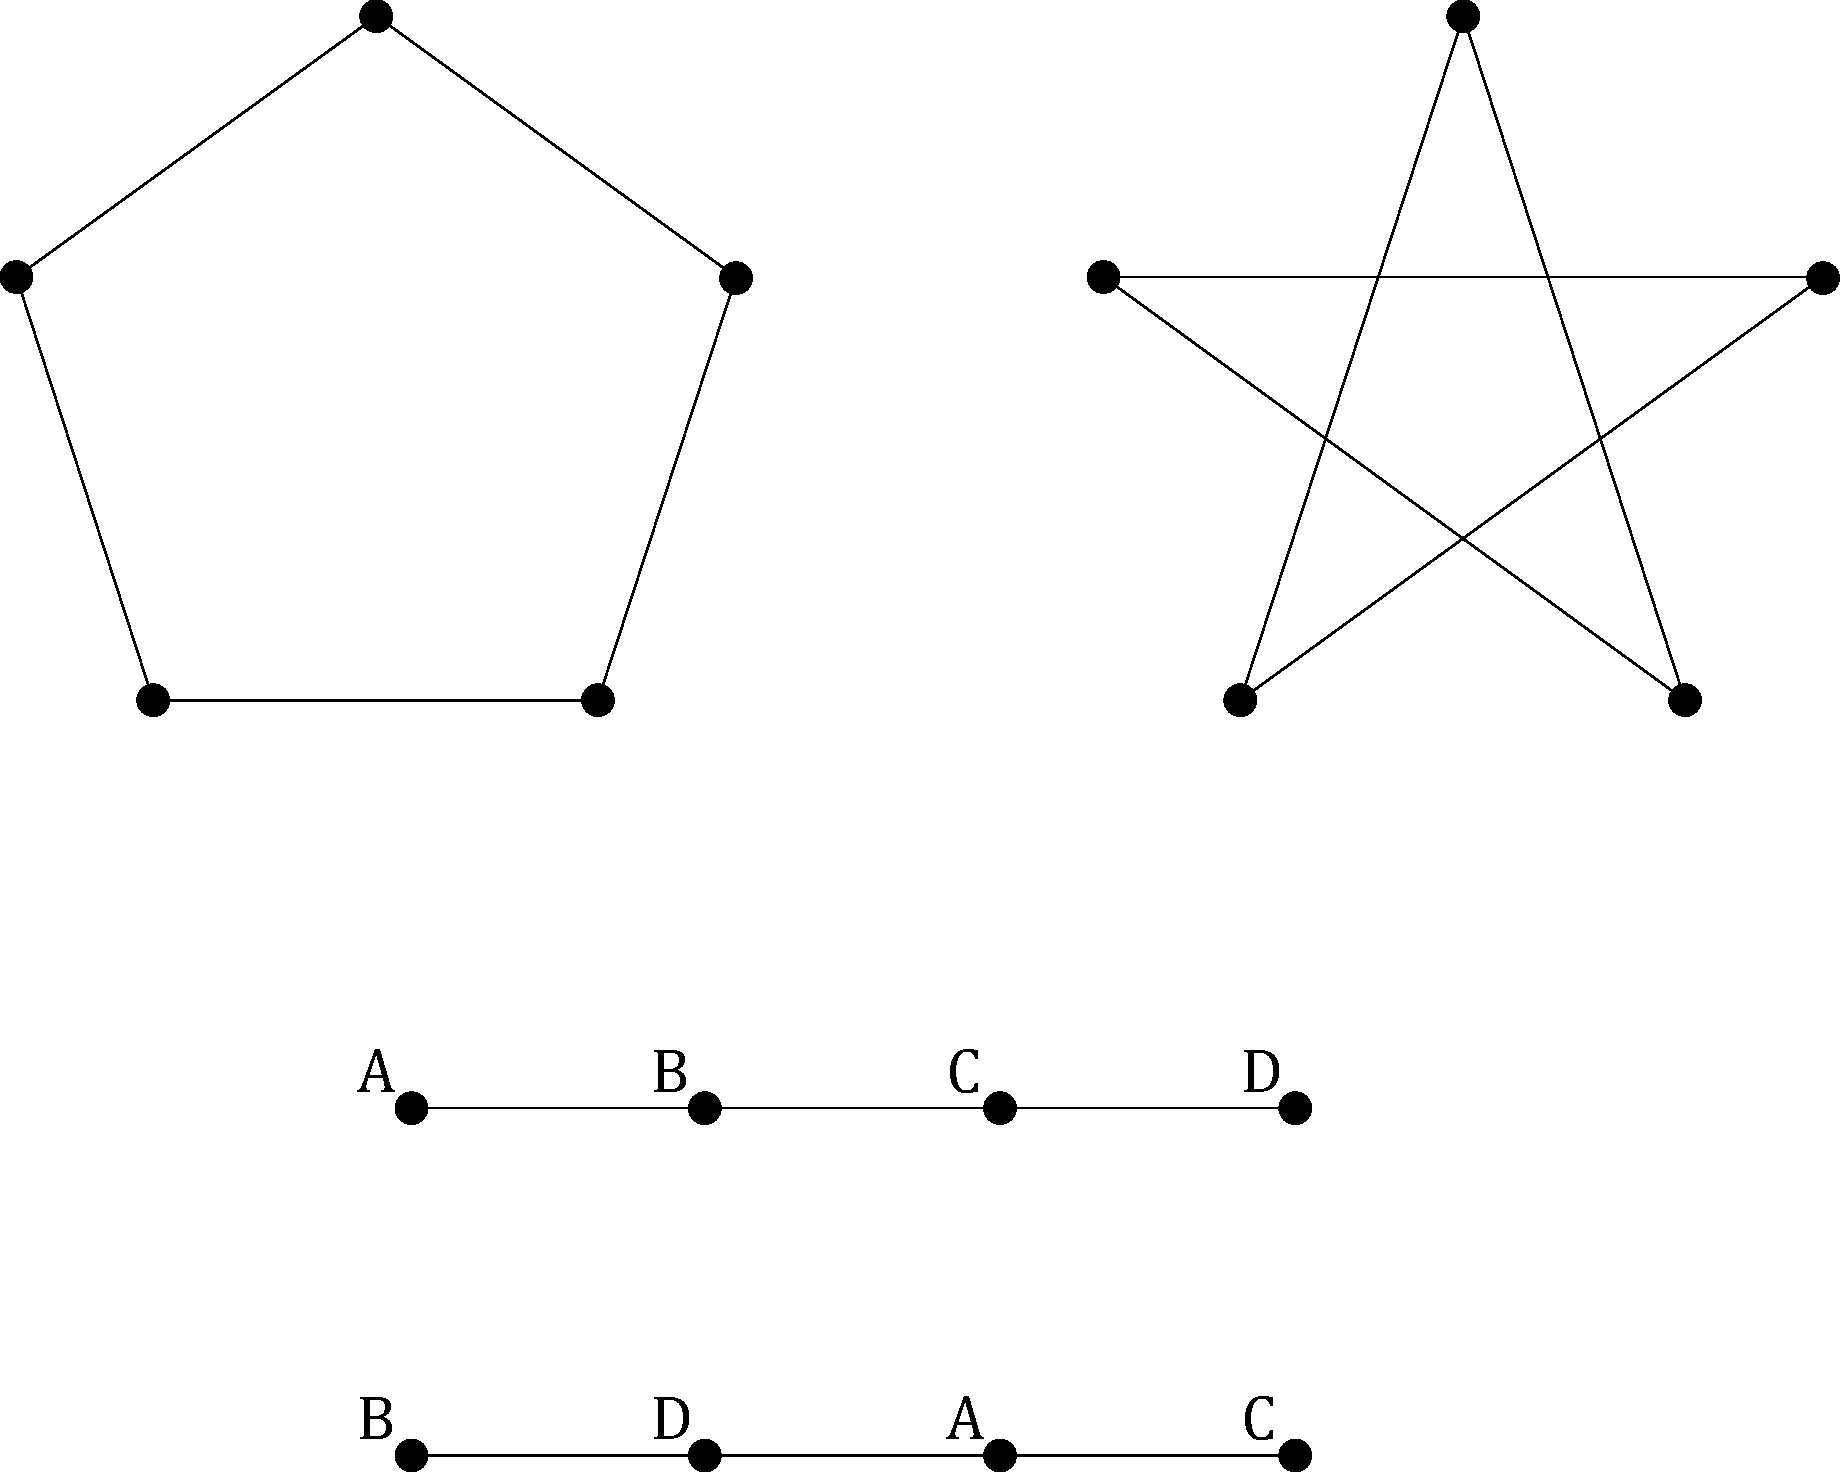
\includegraphics[width = 0.8\textwidth]{2_4_self_compl.pdf}
                    \caption{Self complementary graphs $C_5$, $P_4$}
                    \label{fig:2_4_self_compl}
                \end{figure}
            }
        \end{description}
      }
      \item {
        What is the necessary and sufficient condition for $K_{m,n}$ to be a regular graph?
        
        \begin{description}[leftmargin=0em]
           \item[Answer:] {
                In the complete bipartite graph $K_{m,n}$, the vertices have degree $m$ or degree $n$ (and both of these degrees are reached). Thus, to be regular, a sufficient and necessary condition is $n=m$. \cite{3733224}
            }
        \end{description}
      }
      \item {
        Is there a simple graph of $n$ vertices such that the vertices all have distinct degrees? Give a proof supporting your answer.
        
        \begin{description}[leftmargin=0em]
           \item[Answer:] {
                If $n=1$, yes, trivial. \\
                For $n>1$. Suppose such a graph exists. Each vertex in the graph can have a degree from $0$ to $n-1$ (simple graphs do not forbid a degree-$0$ vertex, \emph{connected} graphs do). Since this range spans $n$ values in total and each vertex degree is different, the degrees are distributed one-per-vertex. In particular, there must exist a vertex with degree $n-1$ and one with degree $0$. \\
                Now the degree-$n-1$ vertex is connected to all other vertices because the graph is simple, \emph{including} the degree-$0$ vertex. But the latter is not connected to any vertex, which is a contradiction. Therefore two vertices in the graph must have the same degree.
                \cite{2690153} \cite{202585439}
            }
        \end{description}
      }
      \item {
        Draw the graph $G = (V, E)$ with vertex set $V = \{a, b, c, d, e, f, g, h\}$ and edge set $\{(a, b), (a, e), (b, c), (b, d), (c, d), (c, g), (d, e)(e, f ), ( f, g), ( f, h), (g, h)\}$. Draw $G - (d, e)$. Draw the subgraph of $G$ induced by $\{c, d, e, f\}$. Contract the edge $(d, e)$ from $G$.
        
        \begin{description}[leftmargin=0em]
           \item[Answer:] {
                Graph drawings Figure \ref{fig:2_7}
                \begin{figure}[ht]
                    \centering
                    \begin{subfigure}[b]{0.4\textwidth}
                        \centering
                        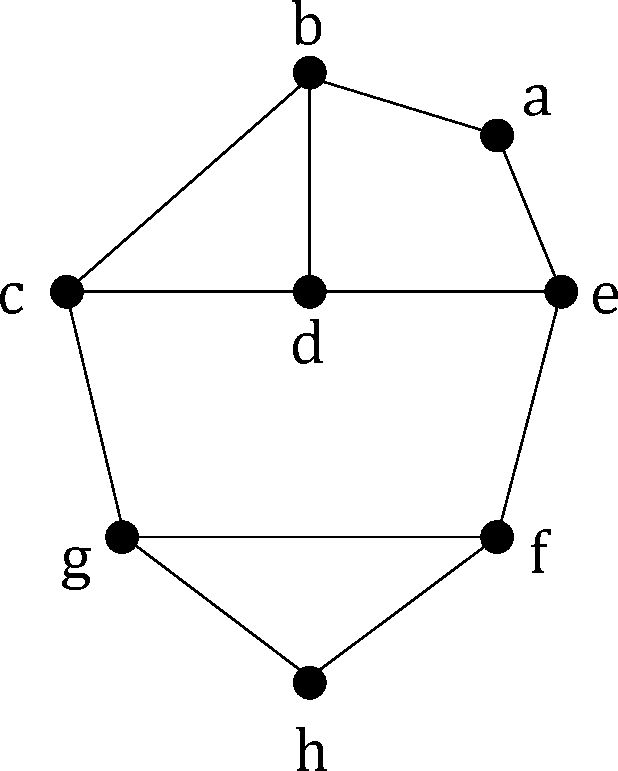
\includegraphics[width = 0.8\textwidth]{2_7_G.pdf}
                        \caption{$G$}
                        \label{fig:2_7_G}
                    \end{subfigure}
                    % \hfill
                    \begin{subfigure}[b]{0.4\textwidth}
                        \centering
                        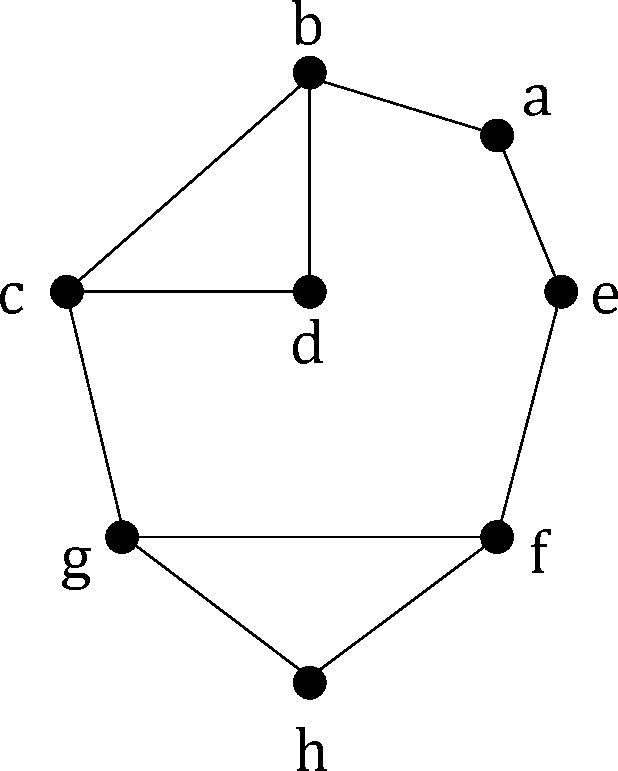
\includegraphics[width = 0.8\textwidth]{2_7_G-d_e.pdf}
                        \caption{$G-(d,e)$}
                        \label{fig:2_7_G-d_e}
                    \end{subfigure}
                    % \hfill
                    \begin{subfigure}[b]{0.4\textwidth}
                        \centering
                        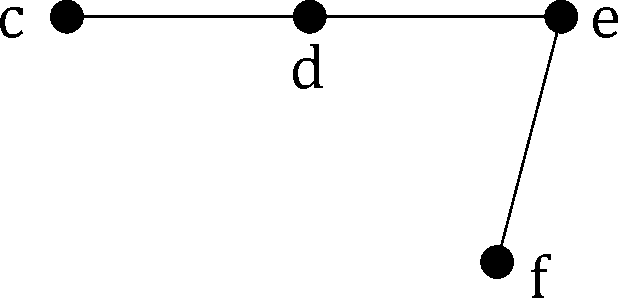
\includegraphics[width = 0.8\textwidth]{2_7_c_d_e_f.pdf}
                        \caption{$G$ induced by $\{c, d, e, f\}$}
                        \label{fig:2_7_c_d_e_f}
                    \end{subfigure}
                    % \hfill
                    \begin{subfigure}[b]{0.4\textwidth}
                        \centering
                        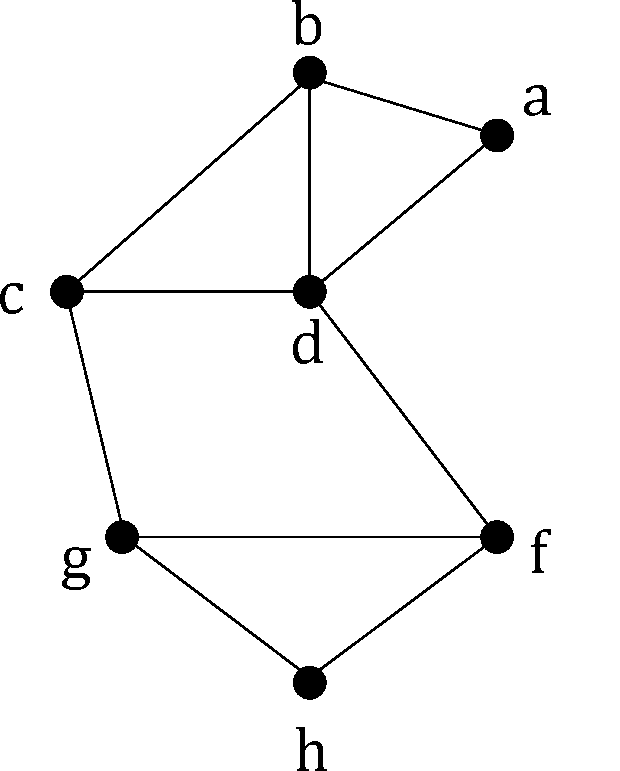
\includegraphics[width = 0.8\textwidth]{2_7_G-d_e_contr.pdf}
                        \caption{$(d, e)$ edge contracted from $G$}
                        \label{fig:2_7_G-d_e_contr}
                    \end{subfigure}
                    
                    \caption{Graph drawings}
                    \label{fig:2_7}
                \end{figure}
            }
        \end{description}
      }
      \item {
        Show that two graphs are isomorphic if and only if their complements are isomorphic.
        
        \begin{description}[leftmargin=0em]
           \item[Answer:] {
                Let graph $G$ be isomorphic to $H$, and let $\overline G$, $\overline H$ denote their complements. \\
                Since $G$ is isomorphic to $H$, then there exists a bijection $f: V(G) \to V(H)$, such that $(u, v) \in E(G)$ if and only if $(f(u), f(v)) \in E(H)$. \\
                Equivalently, there exists a bijection $f: V(G) \to V(H)$, such that $(u, v) \notin E(G)$ if and only if $(f(u), f(v)) \notin E(H)$. \\
                Since the vertex set of $G$ and $\overline G$ are the same, therefore $f$ is a bijection from $V(\overline G)$ to $V(\overline H)$. Then suppose $(u, v) \notin E(G)$, by definition of a complement, $(u, v) \in E(\overline G)$. Likewise, if $(f(u), f(v)) \notin E(H)$, then $(f(u), f(v)) \in E(\overline H)$. \\
                Hence $\overline G$ and $\overline H$ are isomorphic. \cite{2451171}
            }
        \end{description}
      }
    \end{enumerate}
    
% \section{Solutions}
%     \begin{enumerate}[leftmargin=1.5em]
%       \item {
%         % Show that every regular graph with an odd degree has an even number of vertices.
        
%         \begin{description}[leftmargin=0em]
%           \item[Answer:] {
%                 $k$-regular graph of vertices $n$, where $k$ is odd.\\
%                 Degree sum $= 2m$, where $m$ is number of edges.\\
%                 $2m = k \times n$\\
%                 $k$ is odd, $2m$ is even.\\
%                 $\therefore n$ must be even.
%             }
%         \end{description}
%       }
%       \item {
%         % Construct the complement of $K_{3,3}, W_{5}$, and $C_{5}$.
        
%         \begin{description}[leftmargin=0em]
%           \item[Answer:] {
%                 Complement of $K_{3,3}$ Figure \ref{fig:2_2_k}
%                 \begin{figure}[H]
%                     \centering
%                     \begin{subfigure}[b]{0.3\textwidth}
%                         \centering
%                         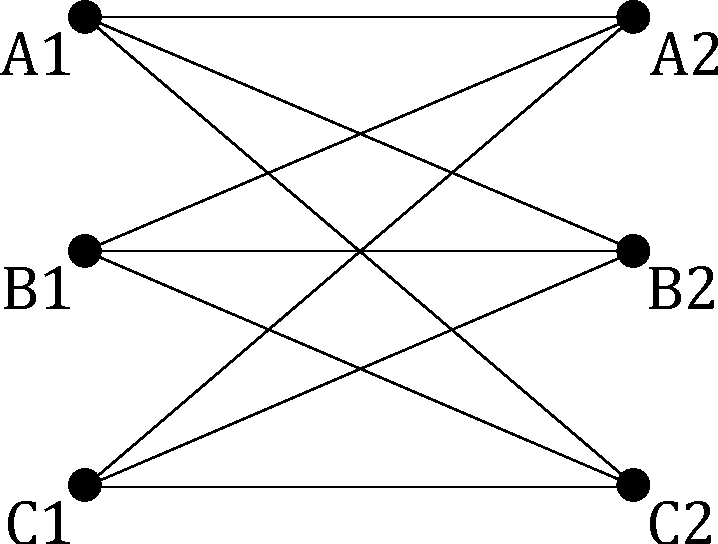
\includegraphics[width = 0.8\textwidth]{2_2_k33.pdf}
%                         \caption{$K_{3,3}$}
%                         \label{fig:2_2_k33}
%                     \end{subfigure}
%                     % \hfill
%                     \begin{subfigure}[b]{0.4\textwidth}
%                         \centering
%                         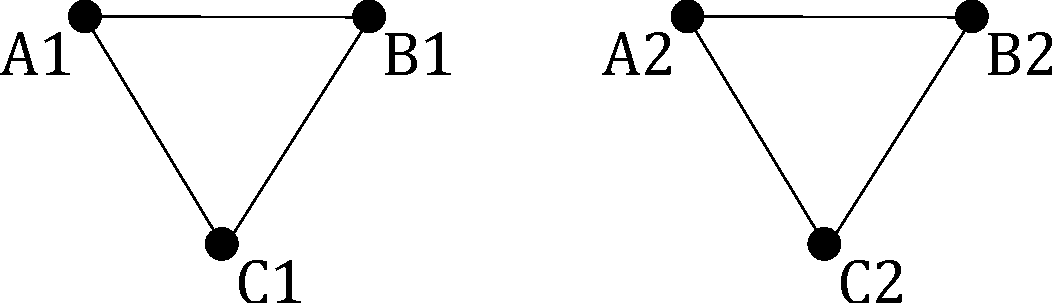
\includegraphics[width = 0.8\textwidth]{2_2_k33_c.pdf}
%                         \caption{$\overline{K}_{3,3}$}
%                         \label{fig:2_2_k33_c}
%                     \end{subfigure}
%                     \caption{Complement of $K_{3,3}$}
%                     \label{fig:2_2_k}
%                 \end{figure}
                
%                 Complement of $W_{5}$ Figure \ref{fig:2_2_w}
%                 \begin{figure}[H]
%                     \centering
%                     \begin{subfigure}[b]{0.3\textwidth}
%                         \centering
%                         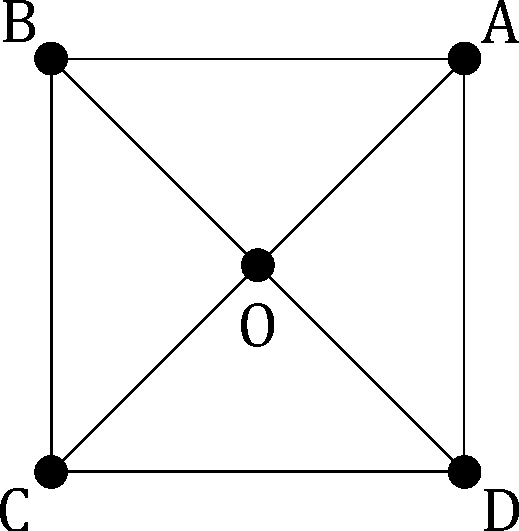
\includegraphics[width = 0.8\textwidth]{2_2_w5.pdf}
%                         \caption{$W_{5}$}
%                         \label{fig:2_2_w5}
%                     \end{subfigure}
%                     % \hfill
%                     \begin{subfigure}[b]{0.4\textwidth}
%                         \centering
%                         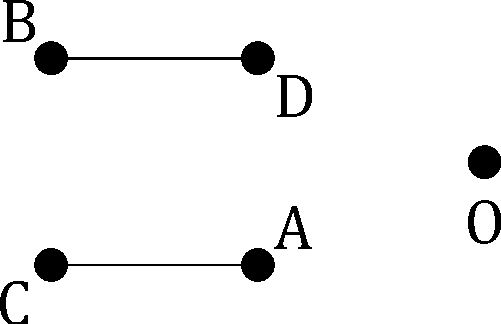
\includegraphics[width = 0.8\textwidth]{2_2_w5_c.pdf}
%                         \caption{$\overline{W}_{5}$}
%                         \label{fig:2_2_w5_c}
%                     \end{subfigure}
%                     \caption{Complement of $W_{5}$}
%                     \label{fig:2_2_w}
%                 \end{figure}
                
%                 Complement of $C_{5}$ Figure \ref{fig:2_2_c}
%                 \begin{figure}[H]
%                     \centering
%                     \begin{subfigure}[b]{0.3\textwidth}
%                         \centering
%                         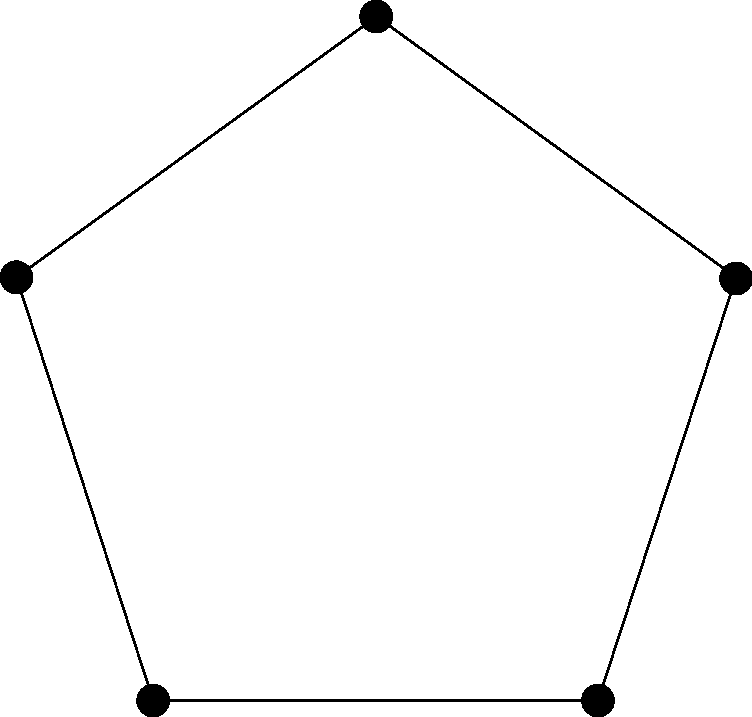
\includegraphics[width = 0.8\textwidth]{2_2_c5.pdf}
%                         \caption{$C_{5}$}
%                         \label{fig:2_2_c5}
%                     \end{subfigure}
%                     % \hfill
%                     \begin{subfigure}[b]{0.3\textwidth}
%                         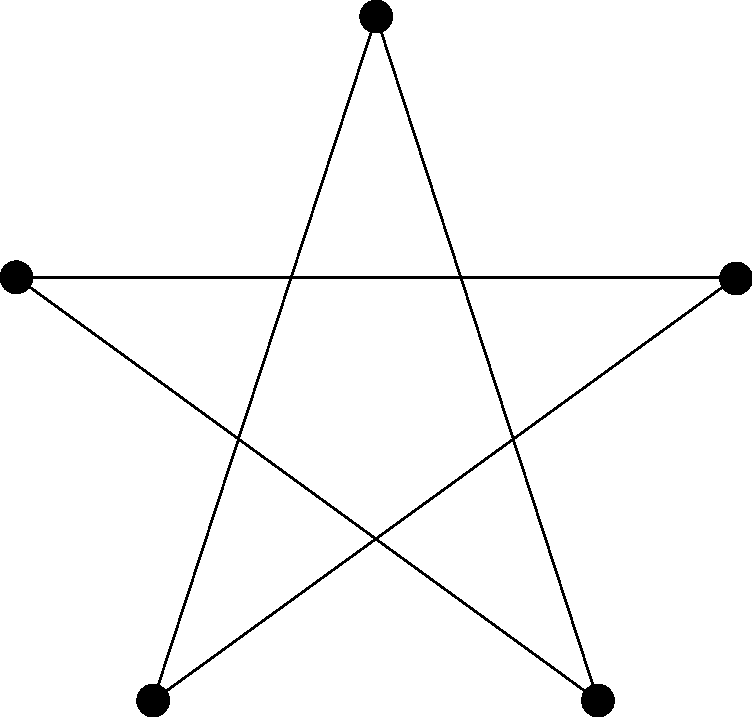
\includegraphics[width = 0.8\textwidth]{2_2_c5_c.pdf}
%                         \caption{$\overline{C}_{5}$}
%                         \label{fig:2_2_c5_c}
%                     \end{subfigure}
%                     \caption{Complement of $C_{5}$}
%                     \label{fig:2_2_c}
%                 \end{figure}
%             }
%         \end{description}
%       }
%       \item {
%         % Can you construct a disconnected graph $G$ of two or more vertices such that $	\overline{G}$ is also disconnected. Give a proof supporting your answer.
        
%         \begin{description}[leftmargin=0em]
%           \item[Answer:] {
%                 No.\\
%                 Let us prove given a graph $G$ of two or more vertices, either $G$ or $\overline{G}$ is connected. \\
%                 $G$ is disconnected. We want to show that $\overline{G}$ is connected. \\
%                 Suppose $v$ and $w$ are vertices. If $(v, w)$ is not an edge in $G$, then it is an edge in $\overline{G}$, and so we have a path from $v$ to $w$ in $\overline{G}$. On the other hand, if $(v, w)$ is an edge in $G$, then this means $v$ and $w$ are in the same component of $G$. Since $G$ is disconnected, we can find a vertex $u$ in a different component, so that neither $(v, u)$ nor $(u, w)$ are edges of $G$. Then $(v, u, w)$ is a path from $v$ to $w$ in $\overline{G}$. \\
%                 This shows that any two vertices in $\overline{G}$ have a path (in fact a path of length one or two) between them in $\overline{G}$, so $\overline{G}$ is connected. \cite{122188}
                
%                 Example Figure \ref{fig:2_3_disc_g}:
%                 \begin{figure}[H]
%                     \centering
%                     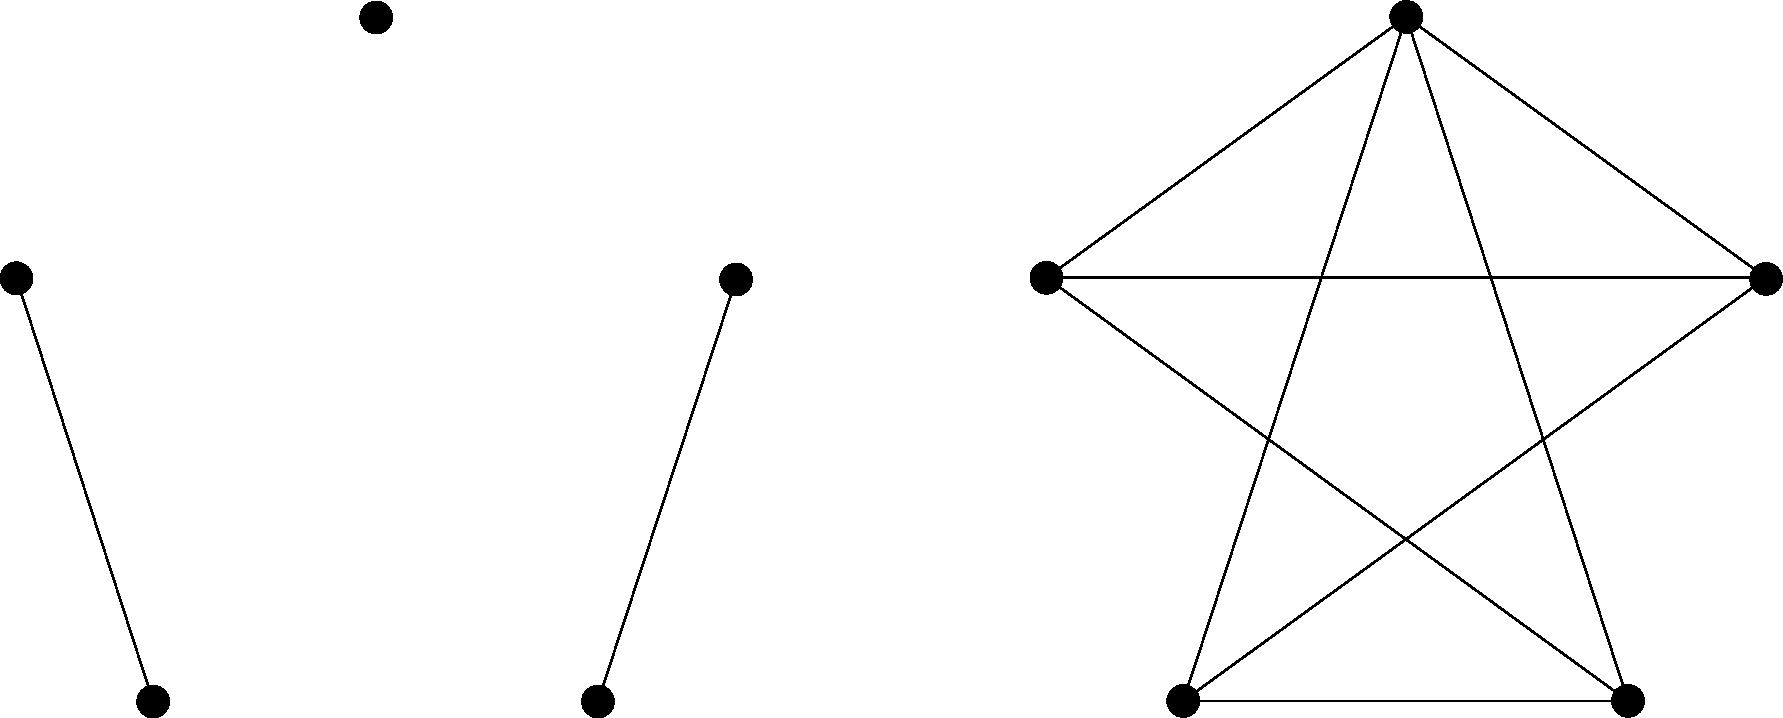
\includegraphics[width = 0.8\textwidth]{2_3_disc_g.pdf}
%                     \caption{Complement of disconnected graph is connected example}
%                     \label{fig:2_3_disc_g}
%                 \end{figure}
%             }
%         \end{description}
%       }
%       \item {
%         % Give two examples of self-complementary graphs.
        
%         \begin{description}[leftmargin=0em]
%           \item[Answer:] {
%                 Self complementary graphs example: $C_5$, $P_4$ Figure \ref{fig:2_4_self_compl}
%                 \begin{figure}[H]
%                     \centering
%                     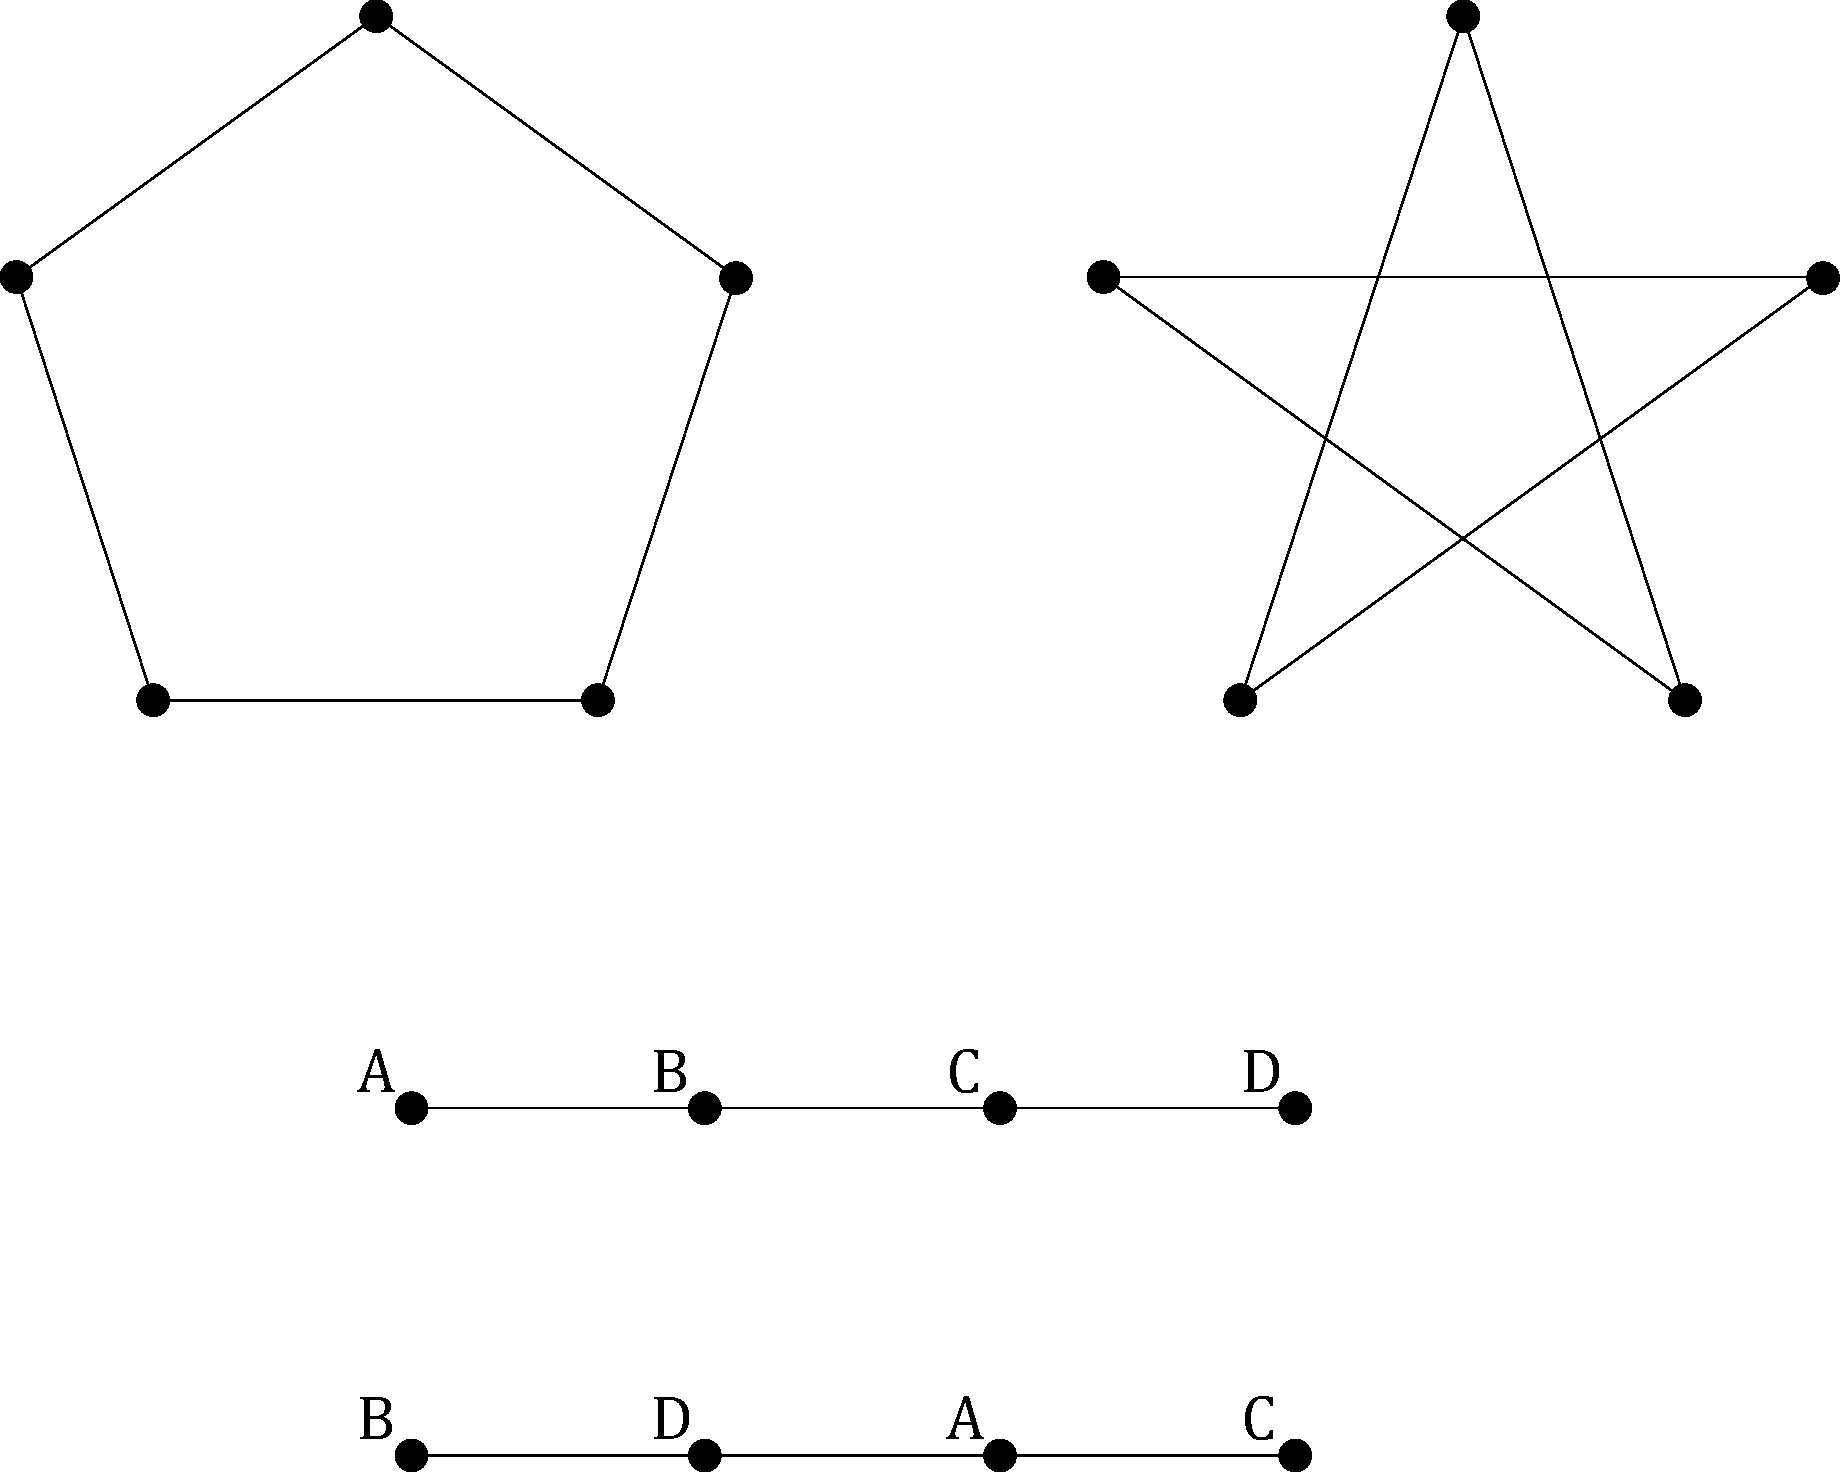
\includegraphics[width = 0.8\textwidth]{2_4_self_compl.pdf}
%                     \caption{Self complementary graphs $C_5$, $P_4$}
%                     \label{fig:2_4_self_compl}
%                 \end{figure}
%             }
%         \end{description}
%       }
%       \item {
%         % What is the necessary and sufficient condition for $K_{m,n}$ to be a regular graph?
        
%         \begin{description}[leftmargin=0em]
%           \item[Answer:] {
%                 In the complete bipartite graph $K_{m,n}$, the vertices have degree $m$ or degree $n$ (and both of these degrees are reached). Thus, to be regular, a sufficient and necessary condition is $n=m$. \cite{3733224}
%             }
%         \end{description}
%       }
%       \item {
%         % Is there a simple graph of $n$ vertices such that the vertices all have distinct degrees? Give a proof supporting your answer.
        
%         \begin{description}[leftmargin=0em]
%           \item[Answer:] {
%                 If $n=1$, yes, trivial. \\
%                 For $n>1$. Suppose such a graph exists. Each vertex in the graph can have a degree from $0$ to $n-1$ (simple graphs do not forbid a degree-$0$ vertex, \emph{connected} graphs do). Since this range spans $n$ values in total and each vertex degree is different, the degrees are distributed one-per-vertex. In particular, there must exist a vertex with degree $n-1$ and one with degree $0$. \\
%                 Now the degree-$n-1$ vertex is connected to all other vertices because the graph is simple, \emph{including} the degree-$0$ vertex. But the latter is not connected to any vertex, which is a contradiction. Therefore two vertices in the graph must have the same degree.
%                 \cite{2690153} \cite{202585439}
%             }
%         \end{description}
%       }
%       \item {
%         % Draw the graph $G = (V, E)$ with vertex set $V = \{a, b, c, d, e, f, g, h\}$ and edge set $\{(a, b), (a, e), (b, c), (b, d), (c, d), (c, g), (d, e)(e, f ), ( f, g), ( f, h), (g, h)\}$. Draw $G - (d, e)$. Draw the subgraph of $G$ induced by $\{c, d, e, f\}$. Contract the edge $(d, e)$ from $G$.
        
%         \begin{description}[leftmargin=0em]
%           \item[Answer:] {
%                 Graph drawings Figure \ref{fig:2_7}
%                 \begin{figure}[ht]
%                     \centering
%                     \begin{subfigure}[b]{0.4\textwidth}
%                         \centering
%                         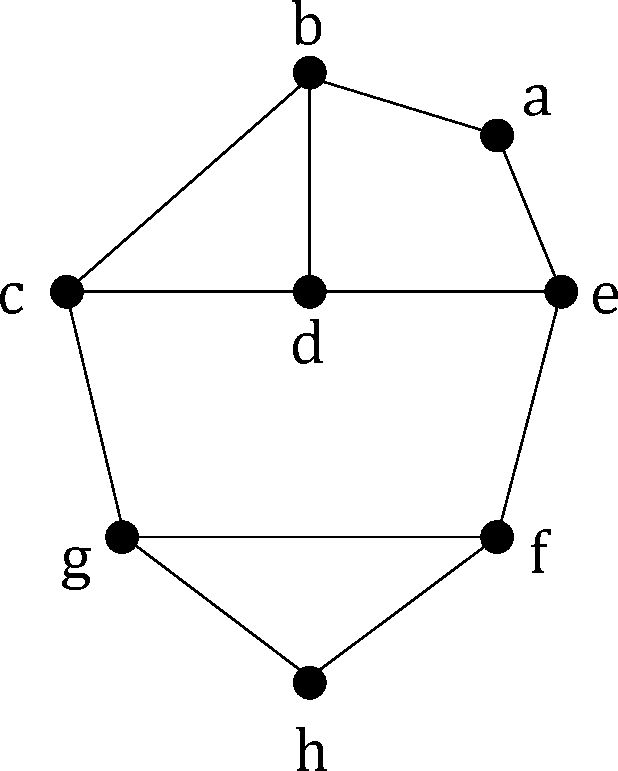
\includegraphics[width = 0.8\textwidth]{2_7_G.pdf}
%                         \caption{$G$}
%                         \label{fig:2_7_G}
%                     \end{subfigure}
%                     % \hfill
%                     \begin{subfigure}[b]{0.4\textwidth}
%                         \centering
%                         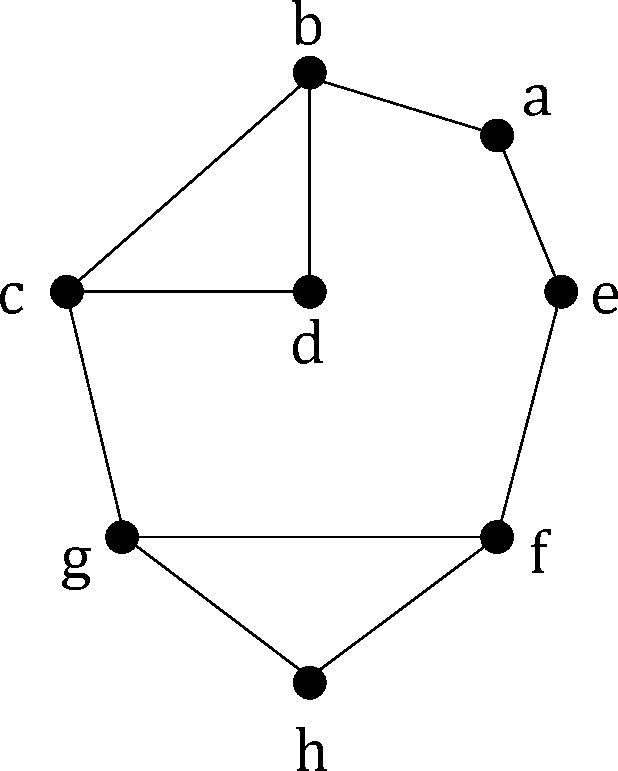
\includegraphics[width = 0.8\textwidth]{2_7_G-d_e.pdf}
%                         \caption{$G-(d,e)$}
%                         \label{fig:2_7_G-d_e}
%                     \end{subfigure}
%                     % \hfill
%                     \begin{subfigure}[b]{0.4\textwidth}
%                         \centering
%                         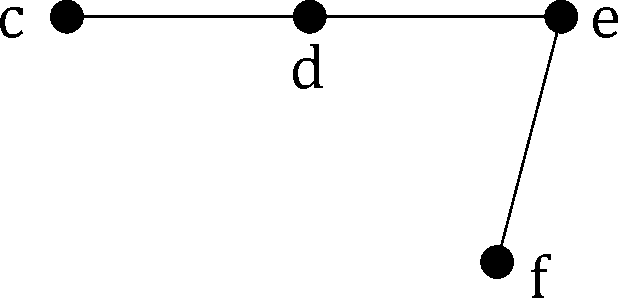
\includegraphics[width = 0.8\textwidth]{2_7_c_d_e_f.pdf}
%                         \caption{$G$ induced by $\{c, d, e, f\}$}
%                         \label{fig:2_7_c_d_e_f}
%                     \end{subfigure}
%                     % \hfill
%                     \begin{subfigure}[b]{0.4\textwidth}
%                         \centering
%                         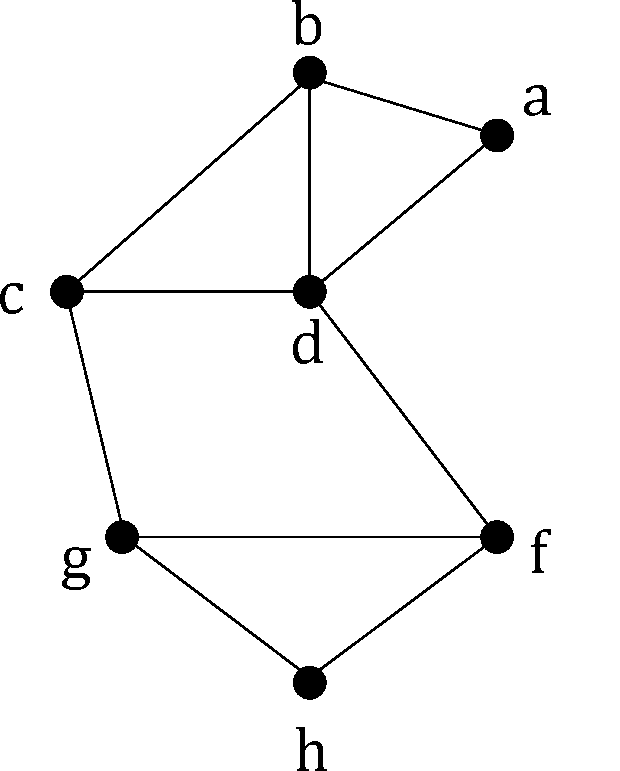
\includegraphics[width = 0.8\textwidth]{2_7_G-d_e_contr.pdf}
%                         \caption{$(d, e)$ edge contracted from $G$}
%                         \label{fig:2_7_G-d_e_contr}
%                     \end{subfigure}
                    
%                     \caption{Graph drawings}
%                     \label{fig:2_7}
%                 \end{figure}
%             }
%         \end{description}
%       }
%       \item {
%         % Show that two graphs are isomorphic if and only if their complements are isomorphic.
        
%         \begin{description}[leftmargin=0em]
%           \item[Answer:] {
%                 Let graph $G$ be isomorphic to $H$, and let $\overline G$, $\overline H$ denote their complements. \\
%                 Since $G$ is isomorphic to $H$, then there exists a bijection $f: V(G) \to V(H)$, such that $(u, v) \in E(G)$ if and only if $(f(u), f(v)) \in E(H)$. \\
%                 Equivalently, there exists a bijection $f: V(G) \to V(H)$, such that $(u, v) \notin E(G)$ if and only if $(f(u), f(v)) \notin E(H)$. \\
%                 Since the vertex set of $G$ and $\overline G$ are the same, therefore $f$ is a bijection from $V(\overline G)$ to $V(\overline H)$. Then suppose $(u, v) \notin E(G)$, by definition of a complement, $(u, v) \in E(\overline G)$. Likewise, if $(f(u), f(v)) \notin E(H)$, then $(f(u), f(v)) \in E(\overline H)$. \\
%                 Hence $\overline G$ and $\overline H$ are isomorphic. \cite{2451171}
%             }
%         \end{description}
%       }
%     \end{enumerate}

%================ch3======================================
\chapter{Paths, Cycles and Connectivity}\label{ch3}
\section{Exercises}

\begin{enumerate}
% 1
    \item {
        Let $G$ be a graph having exactly two vertices $u$ and $v$ of degree three and all other vertices have even degree. Then show that there is an $u, v$-path in $G$ 
        
        \textbf{Answer: } If $u$ and $v$ are in the same component, then the proof is trivial. 
        
        Assume that $u, v$ are in two different components. Let, $u$ belongs to the component $H$. Every other nodes $w \in V(H)-u$ have even degree. So, according to degree-sum theorem, 
        \[ 3 + \sum_{w \in V(H)-u} deg(w) = 2*|E(H)| \]
        But the above equation cannot be true, since $3$ is odd and sum of even degrees is even, which implies that the sum of an odd and even number cannot be even. Which means, $H$ should have even number of \textit{odd degree} nodes (The fact that $H$ should have even number of odd-degree nodes directly follows from \textit{degree-sum theory}). Thus, our assumption of $u$ and $v$ being in two different components is not true.
        
        $\therefore$ There is always a path between $u$ and $v$ as they must belong to the same component
    }
% 2   
    \item {
        Write an algorithm to find a Eulerian circuit in an Eulerian graph based on the sufficiency proof of Lemma 3.2.1
        
        \textbf{Answer:} BFS/DFS using edge coloring. Starting from any vertex $s$, take any unused/uncolored edge from $s$ to go to a neighbour vertex $v$. Color $(s,v)$ so that this edge is not chosen again in the future. Append $s$, $(s,v)$ to the circuit. Recursively perform the algorithm until every edge is colored.
    }
    % 3 
    \item {
        Give a proof of Lemma 3.2.2
        
        \textbf{Answer:} \textit{A connected graph G is Eulerian if and only if G has a cycle decomposition.}
        
        \textit{Proof:} Let $G(V, E)$ be a connected graph and let $G$ be decomposed into cycles. If $k$ of these cycles are incident at a particular vertex $v$, then $d(v) = 2k$. Therefore the degree of every vertex of $G$ is even and hence $G$ is Eulerian.
        
        Conversely, let $G$ be Eulerian. We show $G$ can be decomposed into cycles. To prove this, we use induction on the number of edges.
        
        Since $d(v)\ge 2$ for each $v \in V$, $G$ has a cycle $C$. Then $G-E(C)$ is possibly a disconnected graph, each of whose components $C_1, C_2, ... C_k$ is an even degree graph and hence Eulerian. By the induction hypothesis, each $C_i$ is a disjoint union of cycles. These together with $C$ provide a partition of $E(G)$ into cycles. \cite[p.~65]{tdk_chap_03}
        
        %%%%%%%%%%%%%%%%%%%%%%%% cite this shit
        % http://compalg.inf.elte.hu/~tony/Oktatas/TDK/FINAL/Chap%203.PDF
    }
    % 4
    \item {
        Count the minimum number of edges required to add for making a non-Eulerian graph an Eulerian graph
    
        \textbf{Answer: } Considering the graph to be a simple connected graph, let $x = $ Number of nodes with even degree and $y = $ Number of nodes with odd degree. It follows from \textit{degree-sum theory} that $y$ is even. Pair every two vertexes with odd degree and add an edge between them. Every vertex now have even degree, ensuring an Eulerian graph. Number of edges added was $y/2$
    }
    % 5
    \item {
        Let $K_n$ be a complete graph of $n$ vertices where $n$ is odd and $n \ge 3$. Show that $K_n$ has $(n-1)/2$ edge-disjoint Hamiltonian cycles.
        
        \textbf{Answer:} Since $K_n$ is a complete graph, there exists an edge between any two vertex $v_i$ and $v_j$ for $i \ne j$. Let $n = 2a+1$. We construct the following hamiltonian cycle taking every $(v_i, v_{i+2})$: 
                
        $v_1, v_3, v_5 ... v_{2a+1}, v_2, v_4 ... v_{2a}, v_1$ \\
        $1, 3, 5, ... 2a+1, 2, 4, ... 2a, 1$
        
        Consider the integer sequence representing the cycle. This sequence will not have any repeated element (except $1$) as difference between two element is even and total number of element is odd. There will be repeated element if $GCD($difference, length$) > 1$.
        
        Similarly, we can form a hamiltonian cycles with every even difference.
        
        Difference $2$: $1, 3, 5, ...$ \\
        Difference $4$: $1, 5, 9, ...$ \\
        Difference $6$: $1, 7, 13, ...$
        
        Each difference value represents a unique hamiltonian cycle that shares no edge with each other as neighbours in the integer sequence is different. Valid set of difference values is ${2, 4, ... n-1}$. Thus, there can be $(n-1)/2$ different edge-disjoint hamiltonian cycles.
    }
    % 6
    \item {
        Show that every $k-$regular graph on $2k+1$ vertices is Hamiltonian
    }
    % 7
    \item {
        Write an algorithm to find a pair of vertex disjoint paths between a pair of vertices in a 2-connected graph.
    }
    % 8
    \item {
        Write an algorithm to find an ear decomposition of a biconnected graph
    }
    % 9
    \item {
        Let $s$ be a designated vertex in a connected graph $G = (V, E)$. Design an $O(n+m)$ time algorithm to find a path between $s$ and $v$ with the minimum number of edges for all vertices $v \in V$
        
        \textbf{Answer: } BFS starting from $s$
    }
    % 10
    \item {
        Show that a 3-connected graph has at least six edges
        
        \textbf{Answer:} For a $3$-connected graph, $\kappa(G) \ge 3$. We try to find the minimum number of edges for a graph to be $3$-connected by constructing a graph $G$ with bare minimum number of edges.
        
        From \textit{lemma $3.4.1$}, \textit{$\kappa(G) \leq \delta(G)$}, i.e, the minimum degree of $G$ is 3. Let us thus assume $G$ is a $3$-regular graph, where every vertex has the borderline number of edges. And there must be at least $4$ vertices for every vertex to have $3$ edges. So from construction, we get \textit{$G$ has to be a $3$-regular graph with $4$ vertices}. Such a graph has $6$ edges % edit %
        [from \textit{Corollary $2.2.4$}].
        So, \textit{a 3-connected graph must have at least six edges}
        
        \begin{figure}[H]
            \centering
            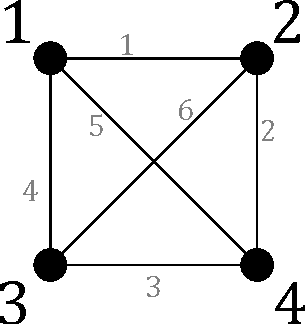
\includegraphics[scale=0.7]{figures/3_10_3-conn-6-edge.pdf} % edit %
            \caption{3-regular graph with 4 vertices}
            \label{fig:3_10}
        \end{figure}
    }
\end{enumerate}

% \include{chapters/chapter_4}
% \include{chapters/chapter_5}

\singlespacing
\renewcommand{\bibname}{References}
\bibliography{bibfile}
	
\end{document}